% =====================================================================================
%  CASSANDRA ML Engine (v1) -- Technical Documentation
%  Compile with pdfLaTeX (Overleaf default). Self-contained: no .bib, no external .tex.
%  Figures: upload docs/figures/v1/*.pdf into a folder "figures/" next to this file.
%  A missing figure is replaced by a framed placeholder, so the document always compiles.
%  Every result number is a macro written by eval/paper_numbers.py (RESULTS block below);
%  a number the results do not provide shows as a red "n/a".
%  The v0 report (4-satellite prototype) is kept in prototype/ml-v0/docs/.
% =====================================================================================
\documentclass[11pt,a4paper]{article}

\usepackage[utf8]{inputenc}
\usepackage[T1]{fontenc}
\usepackage{lmodern}
\usepackage{microtype}
\usepackage[margin=2.2cm]{geometry}
\usepackage{amsmath,amssymb}
\usepackage{graphicx}
\usepackage{booktabs,tabularx,array,multirow}
\usepackage[table]{xcolor}
\usepackage{enumitem}
\usepackage{caption}
\usepackage{float}
\usepackage{tikz}
\usetikzlibrary{arrows.meta,positioning,fit,backgrounds}
\usepackage[colorlinks=true,linkcolor=cblue,citecolor=cblue,urlcolor=cblue]{hyperref}

\definecolor{cblue}{HTML}{2A78D6}
\definecolor{corange}{HTML}{EB6834}
\definecolor{cgreen}{HTML}{1BAF7A}
\definecolor{cviolet}{HTML}{4A3AA7}
\definecolor{cred}{HTML}{D03B3B}
\definecolor{cgray}{HTML}{52514E}
\definecolor{clight}{HTML}{F3F2EE}

\newcommand{\file}[1]{\path{#1}}
\newcommand{\Eeng}{E_{\mathrm{eng}}}
\newcommand{\Esp}{E_{\mathrm{SPARTA}}}
\newcommand{\Elr}{E_{\mathrm{learned}}}
\newcommand{\Eisl}{E_{\mathrm{ISL}}}
\newcommand{\PF}{P(F_s < t+\Delta)}
\newcolumntype{L}{>{\raggedright\arraybackslash}X}

% ----------------------------------------------------------------- RESULTS-BEGIN
% (generated by eval/paper_numbers.py from results/ -- do not edit by hand)
\newcommand{\rActIDAttP}{0.85}
\newcommand{\rActIDAttR}{0.81}
\newcommand{\rActIDAuprc}{0.88}
\newcommand{\rActIDAuroc}{0.999}
\newcommand{\rActIDDelay}{134}
\newcommand{\rActIDEpP}{0.95}
\newcommand{\rActIDEpR}{0.93}
\newcommand{\rActIDFah}{0.02}
\newcommand{\rActIDLead}{38}
\newcommand{\rActIDLeadHi}{41}
\newcommand{\rActIDLeadLo}{34}
\newcommand{\rActIDMean}{36}
\newcommand{\rActIDRec}{0.89}
\newcommand{\rActIDRecHi}{0.93}
\newcommand{\rActIDRecLo}{0.84}
\newcommand{\rActIDVfpr}{0.01}
\newcommand{\rActOODAttP}{0.91}
\newcommand{\rActOODAttR}{0.45}
\newcommand{\rActOODAuprc}{0.73}
\newcommand{\rActOODAuroc}{0.997}
\newcommand{\rActOODDelay}{150}
\newcommand{\rActOODEpP}{0.88}
\newcommand{\rActOODEpR}{0.78}
\newcommand{\rActOODFah}{0.00}
\newcommand{\rActOODLead}{36}
\newcommand{\rActOODLeadHi}{41}
\newcommand{\rActOODLeadLo}{32}
\newcommand{\rActOODMean}{31}
\newcommand{\rActOODRec}{0.73}
\newcommand{\rActOODRecHi}{0.82}
\newcommand{\rActOODRecLo}{0.64}
\newcommand{\rActOODVfpr}{0.00}
\newcommand{\rActRealAttP}{0.76}
\newcommand{\rActRealAttR}{0.78}
\newcommand{\rActRealAuprc}{0.81}
\newcommand{\rActRealAuroc}{0.999}
\newcommand{\rActRealDelay}{178}
\newcommand{\rActRealEpP}{0.87}
\newcommand{\rActRealEpR}{0.84}
\newcommand{\rActRealFah}{0.02}
\newcommand{\rActRealLead}{42}
\newcommand{\rActRealLeadHi}{45}
\newcommand{\rActRealLeadLo}{37}
\newcommand{\rActRealMean}{33}
\newcommand{\rActRealRec}{0.70}
\newcommand{\rActRealRecHi}{0.80}
\newcommand{\rActRealRecLo}{0.59}
\newcommand{\rActRealVfpr}{0.00}
\newcommand{\rAeIDAttP}{0.67}
\newcommand{\rAeIDAttR}{0.84}
\newcommand{\rAeIDAuprc}{0.06}
\newcommand{\rAeIDAuroc}{0.919}
\newcommand{\rAeIDDelay}{9}
\newcommand{\rAeIDEpP}{0.63}
\newcommand{\rAeIDEpR}{0.82}
\newcommand{\rAeIDFah}{0.41}
\newcommand{\rAeIDLead}{187}
\newcommand{\rAeIDLeadHi}{207}
\newcommand{\rAeIDLeadLo}{173}
\newcommand{\rAeIDMean}{66}
\newcommand{\rAeIDPreBurstLead}{182}
\newcommand{\rAeIDPreBurstRec}{0.46}
\newcommand{\rAeIDPreNoneLead}{187}
\newcommand{\rAeIDPreNoneRec}{0.19}
\newcommand{\rAeIDPreSparseLead}{202}
\newcommand{\rAeIDPreSparseRec}{0.32}
\newcommand{\rAeIDRec}{0.34}
\newcommand{\rAeIDRecHi}{0.42}
\newcommand{\rAeIDRecLo}{0.26}
\newcommand{\rAeIDScenALead}{205}
\newcommand{\rAeIDScenARec}{0.49}
\newcommand{\rAeIDScenBLead}{206}
\newcommand{\rAeIDScenBRec}{0.24}
\newcommand{\rAeIDScenCLead}{173}
\newcommand{\rAeIDScenCRec}{0.32}
\newcommand{\rAeIDScenFLead}{--}
\newcommand{\rAeIDScenFRec}{0.00}
\newcommand{\rAeIDVfpr}{0.10}
\newcommand{\rAeOODAttP}{0.72}
\newcommand{\rAeOODAttR}{0.77}
\newcommand{\rAeOODAuprc}{0.04}
\newcommand{\rAeOODAuroc}{0.929}
\newcommand{\rAeOODDelay}{6}
\newcommand{\rAeOODEpP}{0.43}
\newcommand{\rAeOODEpR}{0.83}
\newcommand{\rAeOODFah}{0.30}
\newcommand{\rAeOODLead}{217}
\newcommand{\rAeOODLeadHi}{251}
\newcommand{\rAeOODLeadLo}{166}
\newcommand{\rAeOODMean}{90}
\newcommand{\rAeOODPreBurstLead}{228}
\newcommand{\rAeOODPreBurstRec}{0.27}
\newcommand{\rAeOODPreNoneLead}{182}
\newcommand{\rAeOODPreNoneRec}{0.42}
\newcommand{\rAeOODPreSparseLead}{231}
\newcommand{\rAeOODPreSparseRec}{0.53}
\newcommand{\rAeOODRec}{0.42}
\newcommand{\rAeOODRecHi}{0.52}
\newcommand{\rAeOODRecLo}{0.31}
\newcommand{\rAeOODScenALead}{174}
\newcommand{\rAeOODScenARec}{0.49}
\newcommand{\rAeOODScenBLead}{264}
\newcommand{\rAeOODScenBRec}{0.29}
\newcommand{\rAeOODScenCLead}{235}
\newcommand{\rAeOODScenCRec}{0.48}
\newcommand{\rAeOODScenFLead}{--}
\newcommand{\rAeOODScenFRec}{0.00}
\newcommand{\rAeOODVfpr}{0.08}
\newcommand{\rAeRealAttP}{0.42}
\newcommand{\rAeRealAttR}{0.74}
\newcommand{\rAeRealAuprc}{0.09}
\newcommand{\rAeRealAuroc}{0.957}
\newcommand{\rAeRealDelay}{7}
\newcommand{\rAeRealEpP}{0.45}
\newcommand{\rAeRealEpR}{0.74}
\newcommand{\rAeRealFah}{0.43}
\newcommand{\rAeRealLead}{195}
\newcommand{\rAeRealLeadHi}{223}
\newcommand{\rAeRealLeadLo}{165}
\newcommand{\rAeRealMean}{110}
\newcommand{\rAeRealPreBurstLead}{175}
\newcommand{\rAeRealPreBurstRec}{0.62}
\newcommand{\rAeRealPreNoneLead}{167}
\newcommand{\rAeRealPreNoneRec}{0.44}
\newcommand{\rAeRealPreSparseLead}{211}
\newcommand{\rAeRealPreSparseRec}{0.65}
\newcommand{\rAeRealRec}{0.57}
\newcommand{\rAeRealRecHi}{0.68}
\newcommand{\rAeRealRecLo}{0.45}
\newcommand{\rAeRealScenALead}{204}
\newcommand{\rAeRealScenARec}{0.77}
\newcommand{\rAeRealScenBLead}{196}
\newcommand{\rAeRealScenBRec}{0.60}
\newcommand{\rAeRealScenFLead}{75}
\newcommand{\rAeRealScenFRec}{0.08}
\newcommand{\rAeRealVfpr}{0.11}
\newcommand{\rClAtt}{15}
\newcommand{\rClAvail}{99.95}
\newcommand{\rClAvertAOne}{3}
\newcommand{\rClAvertAThree}{0}
\newcommand{\rClAvertATwo}{2}
\newcommand{\rClAvertBOne}{1}
\newcommand{\rClAvertBTwo}{1}
\newcommand{\rClAvertCOne}{3}
\newcommand{\rClAvertFFive}{1}
\newcommand{\rClAvertFFour}{0}
\newcommand{\rClAvertFTwo}{0}
\newcommand{\rClAvertN}{0}
\newcommand{\rClAverted}{11}
\newcommand{\rClAvertedPct}{61}
\newcommand{\rClBlock}{0}
\newcommand{\rClDecisions}{17}
\newcommand{\rClEp}{24}
\newcommand{\rClFailAOne}{3}
\newcommand{\rClFailAThree}{3}
\newcommand{\rClFailATwo}{2}
\newcommand{\rClFailBOne}{3}
\newcommand{\rClFailBTwo}{1}
\newcommand{\rClFailCOne}{5}
\newcommand{\rClFailFFive}{1}
\newcommand{\rClFailFFour}{0}
\newcommand{\rClFailFTwo}{0}
\newcommand{\rClFailN}{0}
\newcommand{\rClFailWith}{7}
\newcommand{\rClFailWithout}{18}
\newcommand{\rClFalse}{0}
\newcommand{\rClFalsePerOrbit}{0.00}
\newcommand{\rClGated}{0}
\newcommand{\rClIso}{11}
\newcommand{\rClNewFail}{0}
\newcommand{\rClNom}{9}
\newcommand{\rClNoneAOne}{0}
\newcommand{\rClNoneAThree}{0}
\newcommand{\rClNoneATwo}{0}
\newcommand{\rClNoneBOne}{0}
\newcommand{\rClNoneBTwo}{0}
\newcommand{\rClNoneCOne}{51}
\newcommand{\rClNoneFFive}{0}
\newcommand{\rClNoneFFour}{0}
\newcommand{\rClNoneFTwo}{0}
\newcommand{\rClNoneN}{0}
\newcommand{\rClNoneTotal}{51}
\newcommand{\rClPlans}{68}
\newcommand{\rClReroute}{0}
\newcommand{\rClSafe}{6}
\newcommand{\rClStepMs}{161}
\newcommand{\rCucdDrift}{36}
\newcommand{\rCucdLoaoMax}{0.99}
\newcommand{\rCucdLoaoMin}{0.91}
\newcommand{\rCucdShortcut}{99.96}
\newcommand{\rCucdTraffic}{99.99}
\newcommand{\rEceIDCal}{0.002}
\newcommand{\rEceIDSixty}{0.002}
\newcommand{\rEceIDTen}{0.001}
\newcommand{\rEceIDThirty}{0.001}
\newcommand{\rEceIDTwoMin}{0.003}
\newcommand{\rEceOODCal}{0.001}
\newcommand{\rEceOODSixty}{0.001}
\newcommand{\rEceOODTen}{0.000}
\newcommand{\rEceOODThirty}{0.001}
\newcommand{\rEceOODTwoMin}{0.005}
\newcommand{\rEceRealCal}{0.001}
\newcommand{\rEceRealSixty}{0.001}
\newcommand{\rEceRealTen}{0.000}
\newcommand{\rEceRealThirty}{0.001}
\newcommand{\rEceRealTwoMin}{0.003}
\newcommand{\rEnsHSixtyIDAttP}{0.71}
\newcommand{\rEnsHSixtyIDAttR}{0.99}
\newcommand{\rEnsHSixtyIDAuprc}{0.88}
\newcommand{\rEnsHSixtyIDAuroc}{0.999}
\newcommand{\rEnsHSixtyIDDelay}{29}
\newcommand{\rEnsHSixtyIDEpP}{0.70}
\newcommand{\rEnsHSixtyIDEpR}{1.00}
\newcommand{\rEnsHSixtyIDFah}{0.32}
\newcommand{\rEnsHSixtyIDLead}{133}
\newcommand{\rEnsHSixtyIDLeadHi}{140}
\newcommand{\rEnsHSixtyIDLeadLo}{127}
\newcommand{\rEnsHSixtyIDMean}{144}
\newcommand{\rEnsHSixtyIDRec}{1.00}
\newcommand{\rEnsHSixtyIDRecHi}{1.00}
\newcommand{\rEnsHSixtyIDRecLo}{1.00}
\newcommand{\rEnsHSixtyIDVfpr}{0.15}
\newcommand{\rEnsHSixtyOODAttP}{0.78}
\newcommand{\rEnsHSixtyOODAttR}{0.95}
\newcommand{\rEnsHSixtyOODAuprc}{0.73}
\newcommand{\rEnsHSixtyOODAuroc}{0.997}
\newcommand{\rEnsHSixtyOODDelay}{34}
\newcommand{\rEnsHSixtyOODEpP}{0.45}
\newcommand{\rEnsHSixtyOODEpR}{1.00}
\newcommand{\rEnsHSixtyOODFah}{0.28}
\newcommand{\rEnsHSixtyOODLead}{135}
\newcommand{\rEnsHSixtyOODLeadHi}{161}
\newcommand{\rEnsHSixtyOODLeadLo}{128}
\newcommand{\rEnsHSixtyOODMean}{163}
\newcommand{\rEnsHSixtyOODRec}{1.00}
\newcommand{\rEnsHSixtyOODRecHi}{1.00}
\newcommand{\rEnsHSixtyOODRecLo}{1.00}
\newcommand{\rEnsHSixtyOODVfpr}{0.09}
\newcommand{\rEnsHSixtyRealAttP}{0.52}
\newcommand{\rEnsHSixtyRealAttR}{1.00}
\newcommand{\rEnsHSixtyRealAuprc}{0.81}
\newcommand{\rEnsHSixtyRealAuroc}{0.999}
\newcommand{\rEnsHSixtyRealDelay}{30}
\newcommand{\rEnsHSixtyRealEpP}{0.55}
\newcommand{\rEnsHSixtyRealEpR}{1.00}
\newcommand{\rEnsHSixtyRealFah}{0.32}
\newcommand{\rEnsHSixtyRealLead}{162}
\newcommand{\rEnsHSixtyRealLeadHi}{181}
\newcommand{\rEnsHSixtyRealLeadLo}{134}
\newcommand{\rEnsHSixtyRealMean}{169}
\newcommand{\rEnsHSixtyRealRec}{1.00}
\newcommand{\rEnsHSixtyRealRecHi}{1.00}
\newcommand{\rEnsHSixtyRealRecLo}{1.00}
\newcommand{\rEnsHSixtyRealVfpr}{0.15}
\newcommand{\rEnsHTenIDAttP}{0.71}
\newcommand{\rEnsHTenIDAttR}{0.99}
\newcommand{\rEnsHTenIDAuprc}{0.83}
\newcommand{\rEnsHTenIDAuroc}{0.999}
\newcommand{\rEnsHTenIDDelay}{29}
\newcommand{\rEnsHTenIDEpP}{0.70}
\newcommand{\rEnsHTenIDEpR}{1.00}
\newcommand{\rEnsHTenIDFah}{0.33}
\newcommand{\rEnsHTenIDLead}{129}
\newcommand{\rEnsHTenIDLeadHi}{135}
\newcommand{\rEnsHTenIDLeadLo}{122}
\newcommand{\rEnsHTenIDMean}{142}
\newcommand{\rEnsHTenIDRec}{1.00}
\newcommand{\rEnsHTenIDRecHi}{1.00}
\newcommand{\rEnsHTenIDRecLo}{1.00}
\newcommand{\rEnsHTenIDVfpr}{0.16}
\newcommand{\rEnsHTenOODAttP}{0.77}
\newcommand{\rEnsHTenOODAttR}{0.93}
\newcommand{\rEnsHTenOODAuprc}{0.69}
\newcommand{\rEnsHTenOODAuroc}{0.997}
\newcommand{\rEnsHTenOODDelay}{40}
\newcommand{\rEnsHTenOODEpP}{0.46}
\newcommand{\rEnsHTenOODEpR}{1.00}
\newcommand{\rEnsHTenOODFah}{0.30}
\newcommand{\rEnsHTenOODLead}{133}
\newcommand{\rEnsHTenOODLeadHi}{143}
\newcommand{\rEnsHTenOODLeadLo}{121}
\newcommand{\rEnsHTenOODMean}{155}
\newcommand{\rEnsHTenOODRec}{1.00}
\newcommand{\rEnsHTenOODRecHi}{1.00}
\newcommand{\rEnsHTenOODRecLo}{1.00}
\newcommand{\rEnsHTenOODVfpr}{0.09}
\newcommand{\rEnsHTenRealAttP}{0.51}
\newcommand{\rEnsHTenRealAttR}{1.00}
\newcommand{\rEnsHTenRealAuprc}{0.80}
\newcommand{\rEnsHTenRealAuroc}{0.999}
\newcommand{\rEnsHTenRealDelay}{29}
\newcommand{\rEnsHTenRealEpP}{0.54}
\newcommand{\rEnsHTenRealEpR}{1.00}
\newcommand{\rEnsHTenRealFah}{0.33}
\newcommand{\rEnsHTenRealLead}{160}
\newcommand{\rEnsHTenRealLeadHi}{191}
\newcommand{\rEnsHTenRealLeadLo}{136}
\newcommand{\rEnsHTenRealMean}{170}
\newcommand{\rEnsHTenRealRec}{1.00}
\newcommand{\rEnsHTenRealRecHi}{1.00}
\newcommand{\rEnsHTenRealRecLo}{1.00}
\newcommand{\rEnsHTenRealVfpr}{0.15}
\newcommand{\rEnsHThirtyIDAttP}{0.72}
\newcommand{\rEnsHThirtyIDAttR}{0.99}
\newcommand{\rEnsHThirtyIDAuprc}{0.86}
\newcommand{\rEnsHThirtyIDAuroc}{0.999}
\newcommand{\rEnsHThirtyIDDelay}{29}
\newcommand{\rEnsHThirtyIDEpP}{0.70}
\newcommand{\rEnsHThirtyIDEpR}{1.00}
\newcommand{\rEnsHThirtyIDFah}{0.33}
\newcommand{\rEnsHThirtyIDLead}{131}
\newcommand{\rEnsHThirtyIDLeadHi}{137}
\newcommand{\rEnsHThirtyIDLeadLo}{126}
\newcommand{\rEnsHThirtyIDMean}{143}
\newcommand{\rEnsHThirtyIDRec}{1.00}
\newcommand{\rEnsHThirtyIDRecHi}{1.00}
\newcommand{\rEnsHThirtyIDRecLo}{1.00}
\newcommand{\rEnsHThirtyIDVfpr}{0.15}
\newcommand{\rEnsHThirtyOODAttP}{0.78}
\newcommand{\rEnsHThirtyOODAttR}{0.95}
\newcommand{\rEnsHThirtyOODAuprc}{0.71}
\newcommand{\rEnsHThirtyOODAuroc}{0.997}
\newcommand{\rEnsHThirtyOODDelay}{36}
\newcommand{\rEnsHThirtyOODEpP}{0.45}
\newcommand{\rEnsHThirtyOODEpR}{1.00}
\newcommand{\rEnsHThirtyOODFah}{0.29}
\newcommand{\rEnsHThirtyOODLead}{135}
\newcommand{\rEnsHThirtyOODLeadHi}{154}
\newcommand{\rEnsHThirtyOODLeadLo}{124}
\newcommand{\rEnsHThirtyOODMean}{159}
\newcommand{\rEnsHThirtyOODRec}{1.00}
\newcommand{\rEnsHThirtyOODRecHi}{1.00}
\newcommand{\rEnsHThirtyOODRecLo}{1.00}
\newcommand{\rEnsHThirtyOODVfpr}{0.09}
\newcommand{\rEnsHThirtyRealAttP}{0.51}
\newcommand{\rEnsHThirtyRealAttR}{1.00}
\newcommand{\rEnsHThirtyRealAuprc}{0.81}
\newcommand{\rEnsHThirtyRealAuroc}{0.999}
\newcommand{\rEnsHThirtyRealDelay}{29}
\newcommand{\rEnsHThirtyRealEpP}{0.54}
\newcommand{\rEnsHThirtyRealEpR}{1.00}
\newcommand{\rEnsHThirtyRealFah}{0.31}
\newcommand{\rEnsHThirtyRealLead}{165}
\newcommand{\rEnsHThirtyRealLeadHi}{193}
\newcommand{\rEnsHThirtyRealLeadLo}{136}
\newcommand{\rEnsHThirtyRealMean}{170}
\newcommand{\rEnsHThirtyRealRec}{1.00}
\newcommand{\rEnsHThirtyRealRecHi}{1.00}
\newcommand{\rEnsHThirtyRealRecLo}{1.00}
\newcommand{\rEnsHThirtyRealVfpr}{0.15}
\newcommand{\rEnsHTwoMinIDAttP}{0.72}
\newcommand{\rEnsHTwoMinIDAttR}{0.99}
\newcommand{\rEnsHTwoMinIDAuprc}{0.87}
\newcommand{\rEnsHTwoMinIDAuroc}{0.999}
\newcommand{\rEnsHTwoMinIDDelay}{31}
\newcommand{\rEnsHTwoMinIDEpP}{0.71}
\newcommand{\rEnsHTwoMinIDEpR}{1.00}
\newcommand{\rEnsHTwoMinIDFah}{0.32}
\newcommand{\rEnsHTwoMinIDLead}{131}
\newcommand{\rEnsHTwoMinIDLeadHi}{136}
\newcommand{\rEnsHTwoMinIDLeadLo}{126}
\newcommand{\rEnsHTwoMinIDMean}{139}
\newcommand{\rEnsHTwoMinIDRec}{1.00}
\newcommand{\rEnsHTwoMinIDRecHi}{1.00}
\newcommand{\rEnsHTwoMinIDRecLo}{1.00}
\newcommand{\rEnsHTwoMinIDVfpr}{0.14}
\newcommand{\rEnsHTwoMinOODAttP}{0.79}
\newcommand{\rEnsHTwoMinOODAttR}{0.96}
\newcommand{\rEnsHTwoMinOODAuprc}{0.73}
\newcommand{\rEnsHTwoMinOODAuroc}{0.997}
\newcommand{\rEnsHTwoMinOODDelay}{42}
\newcommand{\rEnsHTwoMinOODEpP}{0.46}
\newcommand{\rEnsHTwoMinOODEpR}{1.00}
\newcommand{\rEnsHTwoMinOODFah}{0.27}
\newcommand{\rEnsHTwoMinOODLead}{133}
\newcommand{\rEnsHTwoMinOODLeadHi}{148}
\newcommand{\rEnsHTwoMinOODLeadLo}{124}
\newcommand{\rEnsHTwoMinOODMean}{154}
\newcommand{\rEnsHTwoMinOODRec}{1.00}
\newcommand{\rEnsHTwoMinOODRecHi}{1.00}
\newcommand{\rEnsHTwoMinOODRecLo}{1.00}
\newcommand{\rEnsHTwoMinOODVfpr}{0.08}
\newcommand{\rEnsHTwoMinRealAttP}{0.53}
\newcommand{\rEnsHTwoMinRealAttR}{1.00}
\newcommand{\rEnsHTwoMinRealAuprc}{0.79}
\newcommand{\rEnsHTwoMinRealAuroc}{0.999}
\newcommand{\rEnsHTwoMinRealDelay}{42}
\newcommand{\rEnsHTwoMinRealEpP}{0.57}
\newcommand{\rEnsHTwoMinRealEpR}{1.00}
\newcommand{\rEnsHTwoMinRealFah}{0.30}
\newcommand{\rEnsHTwoMinRealLead}{148}
\newcommand{\rEnsHTwoMinRealLeadHi}{171}
\newcommand{\rEnsHTwoMinRealLeadLo}{124}
\newcommand{\rEnsHTwoMinRealMean}{159}
\newcommand{\rEnsHTwoMinRealRec}{1.00}
\newcommand{\rEnsHTwoMinRealRecHi}{1.00}
\newcommand{\rEnsHTwoMinRealRecLo}{1.00}
\newcommand{\rEnsHTwoMinRealVfpr}{0.14}
\newcommand{\rEnsIDAttP}{0.71}
\newcommand{\rEnsIDAttR}{0.99}
\newcommand{\rEnsIDAuprc}{0.88}
\newcommand{\rEnsIDAuroc}{0.999}
\newcommand{\rEnsIDDelay}{29}
\newcommand{\rEnsIDEpP}{0.70}
\newcommand{\rEnsIDEpR}{1.00}
\newcommand{\rEnsIDFah}{0.32}
\newcommand{\rEnsIDLead}{133}
\newcommand{\rEnsIDLeadHi}{140}
\newcommand{\rEnsIDLeadLo}{127}
\newcommand{\rEnsIDMean}{144}
\newcommand{\rEnsIDPreBurstLead}{139}
\newcommand{\rEnsIDPreBurstRec}{1.00}
\newcommand{\rEnsIDPreNoneLead}{130}
\newcommand{\rEnsIDPreNoneRec}{1.00}
\newcommand{\rEnsIDPreSparseLead}{130}
\newcommand{\rEnsIDPreSparseRec}{1.00}
\newcommand{\rEnsIDRec}{1.00}
\newcommand{\rEnsIDRecHi}{1.00}
\newcommand{\rEnsIDRecLo}{1.00}
\newcommand{\rEnsIDScenALead}{144}
\newcommand{\rEnsIDScenARec}{1.00}
\newcommand{\rEnsIDScenBLead}{163}
\newcommand{\rEnsIDScenBRec}{1.00}
\newcommand{\rEnsIDScenCLead}{127}
\newcommand{\rEnsIDScenCRec}{1.00}
\newcommand{\rEnsIDScenFLead}{108}
\newcommand{\rEnsIDScenFRec}{1.00}
\newcommand{\rEnsIDThresh}{0.02}
\newcommand{\rEnsIDTypeAOneLead}{122}
\newcommand{\rEnsIDTypeAOneN}{28}
\newcommand{\rEnsIDTypeAOneRec}{1.00}
\newcommand{\rEnsIDTypeAThreeLead}{243}
\newcommand{\rEnsIDTypeAThreeN}{16}
\newcommand{\rEnsIDTypeAThreeRec}{1.00}
\newcommand{\rEnsIDTypeATwoLead}{136}
\newcommand{\rEnsIDTypeATwoN}{31}
\newcommand{\rEnsIDTypeATwoRec}{1.00}
\newcommand{\rEnsIDTypeBOneLead}{186}
\newcommand{\rEnsIDTypeBOneN}{15}
\newcommand{\rEnsIDTypeBOneRec}{1.00}
\newcommand{\rEnsIDTypeBTwoLead}{154}
\newcommand{\rEnsIDTypeBTwoN}{14}
\newcommand{\rEnsIDTypeBTwoRec}{1.00}
\newcommand{\rEnsIDTypeCOneLead}{127}
\newcommand{\rEnsIDTypeCOneN}{79}
\newcommand{\rEnsIDTypeCOneRec}{1.00}
\newcommand{\rEnsIDTypeFFiveLead}{108}
\newcommand{\rEnsIDTypeFFiveN}{22}
\newcommand{\rEnsIDTypeFFiveRec}{1.00}
\newcommand{\rEnsIDVfpr}{0.15}
\newcommand{\rEnsLeadMax}{162}
\newcommand{\rEnsLeadMin}{133}
\newcommand{\rEnsOODAttP}{0.78}
\newcommand{\rEnsOODAttR}{0.95}
\newcommand{\rEnsOODAuprc}{0.73}
\newcommand{\rEnsOODAuroc}{0.997}
\newcommand{\rEnsOODDelay}{34}
\newcommand{\rEnsOODEpP}{0.45}
\newcommand{\rEnsOODEpR}{1.00}
\newcommand{\rEnsOODFah}{0.28}
\newcommand{\rEnsOODLead}{135}
\newcommand{\rEnsOODLeadHi}{161}
\newcommand{\rEnsOODLeadLo}{128}
\newcommand{\rEnsOODMean}{163}
\newcommand{\rEnsOODPreBurstLead}{144}
\newcommand{\rEnsOODPreBurstRec}{1.00}
\newcommand{\rEnsOODPreNoneLead}{120}
\newcommand{\rEnsOODPreNoneRec}{1.00}
\newcommand{\rEnsOODPreSparseLead}{174}
\newcommand{\rEnsOODPreSparseRec}{1.00}
\newcommand{\rEnsOODRec}{1.00}
\newcommand{\rEnsOODRecHi}{1.00}
\newcommand{\rEnsOODRecLo}{1.00}
\newcommand{\rEnsOODScenALead}{161}
\newcommand{\rEnsOODScenARec}{1.00}
\newcommand{\rEnsOODScenBLead}{198}
\newcommand{\rEnsOODScenBRec}{1.00}
\newcommand{\rEnsOODScenCLead}{128}
\newcommand{\rEnsOODScenCRec}{1.00}
\newcommand{\rEnsOODScenFLead}{115}
\newcommand{\rEnsOODScenFRec}{1.00}
\newcommand{\rEnsOODTypeAOneLead}{118}
\newcommand{\rEnsOODTypeAOneN}{18}
\newcommand{\rEnsOODTypeAOneRec}{1.00}
\newcommand{\rEnsOODTypeAThreeLead}{275}
\newcommand{\rEnsOODTypeAThreeN}{6}
\newcommand{\rEnsOODTypeAThreeRec}{1.00}
\newcommand{\rEnsOODTypeATwoLead}{182}
\newcommand{\rEnsOODTypeATwoN}{17}
\newcommand{\rEnsOODTypeATwoRec}{1.00}
\newcommand{\rEnsOODTypeBOneLead}{206}
\newcommand{\rEnsOODTypeBOneN}{10}
\newcommand{\rEnsOODTypeBOneRec}{1.00}
\newcommand{\rEnsOODTypeBTwoLead}{196}
\newcommand{\rEnsOODTypeBTwoN}{7}
\newcommand{\rEnsOODTypeBTwoRec}{1.00}
\newcommand{\rEnsOODTypeCOneLead}{128}
\newcommand{\rEnsOODTypeCOneN}{46}
\newcommand{\rEnsOODTypeCOneRec}{1.00}
\newcommand{\rEnsOODTypeFFiveLead}{115}
\newcommand{\rEnsOODTypeFFiveN}{9}
\newcommand{\rEnsOODTypeFFiveRec}{1.00}
\newcommand{\rEnsOODVfpr}{0.09}
\newcommand{\rEnsRealAttP}{0.52}
\newcommand{\rEnsRealAttR}{1.00}
\newcommand{\rEnsRealAuprc}{0.81}
\newcommand{\rEnsRealAuroc}{0.999}
\newcommand{\rEnsRealDelay}{30}
\newcommand{\rEnsRealEpP}{0.55}
\newcommand{\rEnsRealEpR}{1.00}
\newcommand{\rEnsRealFah}{0.32}
\newcommand{\rEnsRealLead}{162}
\newcommand{\rEnsRealLeadHi}{181}
\newcommand{\rEnsRealLeadLo}{134}
\newcommand{\rEnsRealMean}{169}
\newcommand{\rEnsRealPreBurstLead}{150}
\newcommand{\rEnsRealPreBurstRec}{1.00}
\newcommand{\rEnsRealPreNoneLead}{165}
\newcommand{\rEnsRealPreNoneRec}{1.00}
\newcommand{\rEnsRealPreSparseLead}{172}
\newcommand{\rEnsRealPreSparseRec}{1.00}
\newcommand{\rEnsRealRec}{1.00}
\newcommand{\rEnsRealRecHi}{1.00}
\newcommand{\rEnsRealRecLo}{1.00}
\newcommand{\rEnsRealScenALead}{118}
\newcommand{\rEnsRealScenARec}{1.00}
\newcommand{\rEnsRealScenBLead}{204}
\newcommand{\rEnsRealScenBRec}{1.00}
\newcommand{\rEnsRealScenFLead}{109}
\newcommand{\rEnsRealScenFRec}{1.00}
\newcommand{\rEnsRealTypeAOneLead}{118}
\newcommand{\rEnsRealTypeAOneN}{26}
\newcommand{\rEnsRealTypeAOneRec}{1.00}
\newcommand{\rEnsRealTypeBOneLead}{204}
\newcommand{\rEnsRealTypeBOneN}{30}
\newcommand{\rEnsRealTypeBOneRec}{1.00}
\newcommand{\rEnsRealTypeFFiveLead}{109}
\newcommand{\rEnsRealTypeFFiveN}{13}
\newcommand{\rEnsRealTypeFFiveRec}{1.00}
\newcommand{\rEnsRealVfpr}{0.15}
\newcommand{\rFigAlertDelay}{6}
\newcommand{\rFigEpisode}{test\_id-00112}
\newcommand{\rFigFallBefore}{21}
\newcommand{\rGdnIDAttP}{0.56}
\newcommand{\rGdnIDAttR}{1.00}
\newcommand{\rGdnIDAuprc}{0.02}
\newcommand{\rGdnIDAuroc}{0.839}
\newcommand{\rGdnIDDelay}{2}
\newcommand{\rGdnIDEpP}{0.54}
\newcommand{\rGdnIDEpR}{1.00}
\newcommand{\rGdnIDFah}{6.73}
\newcommand{\rGdnIDLead}{167}
\newcommand{\rGdnIDLeadHi}{179}
\newcommand{\rGdnIDLeadLo}{151}
\newcommand{\rGdnIDMean}{116}
\newcommand{\rGdnIDPreBurstLead}{172}
\newcommand{\rGdnIDPreBurstRec}{0.75}
\newcommand{\rGdnIDPreNoneLead}{164}
\newcommand{\rGdnIDPreNoneRec}{0.53}
\newcommand{\rGdnIDPreSparseLead}{162}
\newcommand{\rGdnIDPreSparseRec}{0.74}
\newcommand{\rGdnIDRec}{0.68}
\newcommand{\rGdnIDRecHi}{0.75}
\newcommand{\rGdnIDRecLo}{0.62}
\newcommand{\rGdnIDScenALead}{172}
\newcommand{\rGdnIDScenARec}{0.63}
\newcommand{\rGdnIDScenBLead}{163}
\newcommand{\rGdnIDScenBRec}{0.86}
\newcommand{\rGdnIDScenCLead}{166}
\newcommand{\rGdnIDScenCRec}{0.82}
\newcommand{\rGdnIDScenFLead}{130}
\newcommand{\rGdnIDScenFRec}{0.14}
\newcommand{\rGdnIDVfpr}{0.19}
\newcommand{\rGdnOODAttP}{0.54}
\newcommand{\rGdnOODAttR}{1.00}
\newcommand{\rGdnOODAuprc}{0.01}
\newcommand{\rGdnOODAuroc}{0.841}
\newcommand{\rGdnOODDelay}{2}
\newcommand{\rGdnOODEpP}{0.30}
\newcommand{\rGdnOODEpR}{1.00}
\newcommand{\rGdnOODFah}{6.92}
\newcommand{\rGdnOODLead}{175}
\newcommand{\rGdnOODLeadHi}{226}
\newcommand{\rGdnOODLeadLo}{161}
\newcommand{\rGdnOODMean}{147}
\newcommand{\rGdnOODPreBurstLead}{193}
\newcommand{\rGdnOODPreBurstRec}{0.73}
\newcommand{\rGdnOODPreNoneLead}{156}
\newcommand{\rGdnOODPreNoneRec}{0.65}
\newcommand{\rGdnOODPreSparseLead}{218}
\newcommand{\rGdnOODPreSparseRec}{0.78}
\newcommand{\rGdnOODRec}{0.73}
\newcommand{\rGdnOODRecHi}{0.80}
\newcommand{\rGdnOODRecLo}{0.65}
\newcommand{\rGdnOODScenALead}{166}
\newcommand{\rGdnOODScenARec}{0.66}
\newcommand{\rGdnOODScenBLead}{216}
\newcommand{\rGdnOODScenBRec}{0.88}
\newcommand{\rGdnOODScenCLead}{212}
\newcommand{\rGdnOODScenCRec}{0.80}
\newcommand{\rGdnOODScenFLead}{42}
\newcommand{\rGdnOODScenFRec}{0.33}
\newcommand{\rGdnOODVfpr}{0.19}
\newcommand{\rGdnRealAttP}{0.33}
\newcommand{\rGdnRealAttR}{1.00}
\newcommand{\rGdnRealAuprc}{0.01}
\newcommand{\rGdnRealAuroc}{0.870}
\newcommand{\rGdnRealDelay}{0}
\newcommand{\rGdnRealEpP}{0.34}
\newcommand{\rGdnRealEpR}{1.00}
\newcommand{\rGdnRealFah}{6.98}
\newcommand{\rGdnRealLead}{190}
\newcommand{\rGdnRealLeadHi}{246}
\newcommand{\rGdnRealLeadLo}{163}
\newcommand{\rGdnRealMean}{145}
\newcommand{\rGdnRealPreBurstLead}{169}
\newcommand{\rGdnRealPreBurstRec}{0.90}
\newcommand{\rGdnRealPreNoneLead}{160}
\newcommand{\rGdnRealPreNoneRec}{0.44}
\newcommand{\rGdnRealPreSparseLead}{233}
\newcommand{\rGdnRealPreSparseRec}{0.87}
\newcommand{\rGdnRealRec}{0.72}
\newcommand{\rGdnRealRecHi}{0.83}
\newcommand{\rGdnRealRecLo}{0.62}
\newcommand{\rGdnRealScenALead}{220}
\newcommand{\rGdnRealScenARec}{1.00}
\newcommand{\rGdnRealScenBLead}{190}
\newcommand{\rGdnRealScenBRec}{0.70}
\newcommand{\rGdnRealScenFLead}{79}
\newcommand{\rGdnRealScenFRec}{0.23}
\newcommand{\rGdnRealVfpr}{0.19}
\newcommand{\rLatPlan}{1310}
\newcommand{\rLatPlanMax}{1874}
\newcommand{\rLatPlanMin}{512}
\newcommand{\rLatPlanP}{1476}
\newcommand{\rLatPlanRatio}{8.7}
\newcommand{\rLatStep}{30.6}
\newcommand{\rLatStepFour}{39.5}
\newcommand{\rLatStepP}{55.2}
\newcommand{\rMalIDAcc}{90}
\newcommand{\rMalIDAuroc}{0.954}
\newcommand{\rMalOODAcc}{91}
\newcommand{\rMalOODAuroc}{0.940}
\newcommand{\rMalRealAcc}{86}
\newcommand{\rMalRealAuroc}{0.935}
\newcommand{\rMaskShareID}{14}
\newcommand{\rMaskShareOOD}{15}
\newcommand{\rMaskShareReal}{43}
\newcommand{\rNextIDTop}{86}
\newcommand{\rNextIDTopThree}{99}
\newcommand{\rNextOODTop}{84}
\newcommand{\rNextOODTopThree}{99}
\newcommand{\rNextRealTop}{24}
\newcommand{\rNextRealTopThree}{81}
\newcommand{\rNfailID}{205}
\newcommand{\rNfailOOD}{113}
\newcommand{\rNfailReal}{69}
\newcommand{\rNoEngIDAttP}{0.72}
\newcommand{\rNoEngIDAttR}{0.99}
\newcommand{\rNoEngIDAuprc}{0.86}
\newcommand{\rNoEngIDAuroc}{0.999}
\newcommand{\rNoEngIDDelay}{29}
\newcommand{\rNoEngIDEpP}{0.70}
\newcommand{\rNoEngIDEpR}{1.00}
\newcommand{\rNoEngIDFah}{0.43}
\newcommand{\rNoEngIDLead}{133}
\newcommand{\rNoEngIDLeadHi}{139}
\newcommand{\rNoEngIDLeadLo}{128}
\newcommand{\rNoEngIDMean}{143}
\newcommand{\rNoEngIDPreBurstLead}{135}
\newcommand{\rNoEngIDPreBurstRec}{1.00}
\newcommand{\rNoEngIDPreNoneLead}{129}
\newcommand{\rNoEngIDPreNoneRec}{1.00}
\newcommand{\rNoEngIDPreSparseLead}{130}
\newcommand{\rNoEngIDPreSparseRec}{1.00}
\newcommand{\rNoEngIDRec}{1.00}
\newcommand{\rNoEngIDRecHi}{1.00}
\newcommand{\rNoEngIDRecLo}{1.00}
\newcommand{\rNoEngIDScenALead}{141}
\newcommand{\rNoEngIDScenARec}{1.00}
\newcommand{\rNoEngIDScenBLead}{160}
\newcommand{\rNoEngIDScenBRec}{1.00}
\newcommand{\rNoEngIDScenCLead}{130}
\newcommand{\rNoEngIDScenCRec}{1.00}
\newcommand{\rNoEngIDScenFLead}{100}
\newcommand{\rNoEngIDScenFRec}{1.00}
\newcommand{\rNoEngIDVfpr}{0.14}
\newcommand{\rNoEngRealAttP}{0.54}
\newcommand{\rNoEngRealAttR}{1.00}
\newcommand{\rNoEngRealAuprc}{0.81}
\newcommand{\rNoEngRealAuroc}{0.999}
\newcommand{\rNoEngRealDelay}{33}
\newcommand{\rNoEngRealEpP}{0.57}
\newcommand{\rNoEngRealEpR}{1.00}
\newcommand{\rNoEngRealFah}{0.36}
\newcommand{\rNoEngRealLead}{158}
\newcommand{\rNoEngRealLeadHi}{181}
\newcommand{\rNoEngRealLeadLo}{131}
\newcommand{\rNoEngRealMean}{166}
\newcommand{\rNoEngRealPreBurstLead}{152}
\newcommand{\rNoEngRealPreBurstRec}{1.00}
\newcommand{\rNoEngRealPreNoneLead}{145}
\newcommand{\rNoEngRealPreNoneRec}{1.00}
\newcommand{\rNoEngRealPreSparseLead}{170}
\newcommand{\rNoEngRealPreSparseRec}{1.00}
\newcommand{\rNoEngRealRec}{1.00}
\newcommand{\rNoEngRealRecHi}{1.00}
\newcommand{\rNoEngRealRecLo}{1.00}
\newcommand{\rNoEngRealScenALead}{118}
\newcommand{\rNoEngRealScenARec}{1.00}
\newcommand{\rNoEngRealScenBLead}{204}
\newcommand{\rNoEngRealScenBRec}{1.00}
\newcommand{\rNoEngRealScenFLead}{96}
\newcommand{\rNoEngRealScenFRec}{1.00}
\newcommand{\rNoEngRealVfpr}{0.15}
\newcommand{\rNoResIDAttP}{0.71}
\newcommand{\rNoResIDAttR}{0.99}
\newcommand{\rNoResIDAuprc}{0.84}
\newcommand{\rNoResIDAuroc}{0.999}
\newcommand{\rNoResIDDelay}{27}
\newcommand{\rNoResIDEpP}{0.69}
\newcommand{\rNoResIDEpR}{1.00}
\newcommand{\rNoResIDFah}{0.34}
\newcommand{\rNoResIDLead}{132}
\newcommand{\rNoResIDLeadHi}{138}
\newcommand{\rNoResIDLeadLo}{124}
\newcommand{\rNoResIDMean}{142}
\newcommand{\rNoResIDPreBurstLead}{137}
\newcommand{\rNoResIDPreBurstRec}{1.00}
\newcommand{\rNoResIDPreNoneLead}{124}
\newcommand{\rNoResIDPreNoneRec}{1.00}
\newcommand{\rNoResIDPreSparseLead}{128}
\newcommand{\rNoResIDPreSparseRec}{1.00}
\newcommand{\rNoResIDRec}{1.00}
\newcommand{\rNoResIDRecHi}{1.00}
\newcommand{\rNoResIDRecLo}{1.00}
\newcommand{\rNoResIDScenALead}{142}
\newcommand{\rNoResIDScenARec}{1.00}
\newcommand{\rNoResIDScenBLead}{163}
\newcommand{\rNoResIDScenBRec}{1.00}
\newcommand{\rNoResIDScenCLead}{125}
\newcommand{\rNoResIDScenCRec}{1.00}
\newcommand{\rNoResIDScenFLead}{102}
\newcommand{\rNoResIDScenFRec}{1.00}
\newcommand{\rNoResIDVfpr}{0.13}
\newcommand{\rNoResRealAttP}{0.53}
\newcommand{\rNoResRealAttR}{1.00}
\newcommand{\rNoResRealAuprc}{0.78}
\newcommand{\rNoResRealAuroc}{0.999}
\newcommand{\rNoResRealDelay}{27}
\newcommand{\rNoResRealEpP}{0.57}
\newcommand{\rNoResRealEpR}{1.00}
\newcommand{\rNoResRealFah}{0.32}
\newcommand{\rNoResRealLead}{160}
\newcommand{\rNoResRealLeadHi}{182}
\newcommand{\rNoResRealLeadLo}{126}
\newcommand{\rNoResRealMean}{167}
\newcommand{\rNoResRealPreBurstLead}{150}
\newcommand{\rNoResRealPreBurstRec}{1.00}
\newcommand{\rNoResRealPreNoneLead}{154}
\newcommand{\rNoResRealPreNoneRec}{1.00}
\newcommand{\rNoResRealPreSparseLead}{179}
\newcommand{\rNoResRealPreSparseRec}{1.00}
\newcommand{\rNoResRealRec}{1.00}
\newcommand{\rNoResRealRecHi}{1.00}
\newcommand{\rNoResRealRecLo}{1.00}
\newcommand{\rNoResRealScenALead}{118}
\newcommand{\rNoResRealScenARec}{1.00}
\newcommand{\rNoResRealScenBLead}{204}
\newcommand{\rNoResRealScenBRec}{1.00}
\newcommand{\rNoResRealScenFLead}{99}
\newcommand{\rNoResRealScenFRec}{1.00}
\newcommand{\rNoResRealVfpr}{0.14}
\newcommand{\rNtestEp}{800}
\newcommand{\rQgateID}{0.005}
\newcommand{\rQgateOOD}{0.036}
\newcommand{\rQgateReal}{0.006}
\newcommand{\rQmedID}{0.000}
\newcommand{\rQmedOOD}{0.000}
\newcommand{\rQmedReal}{0.000}
\newcommand{\rRobALead}{183}
\newcommand{\rRobAQ}{0.14}
\newcommand{\rRobARec}{0.92}
\newcommand{\rRobAThrLead}{36}
\newcommand{\rRobAThrRec}{0.83}
\newcommand{\rRobBLead}{198}
\newcommand{\rRobBQ}{0.16}
\newcommand{\rRobBRec}{1.00}
\newcommand{\rRobBThrLead}{32}
\newcommand{\rRobBThrRec}{0.83}
\newcommand{\rRobCLead}{199}
\newcommand{\rRobCQ}{0.19}
\newcommand{\rRobCRec}{1.00}
\newcommand{\rRobCThrLead}{24}
\newcommand{\rRobCThrRec}{0.83}
\newcommand{\rRobN}{12}
\newcommand{\rRobZeroLead}{146}
\newcommand{\rRobZeroQ}{0.10}
\newcommand{\rRobZeroRec}{1.00}
\newcommand{\rRobZeroThrLead}{40}
\newcommand{\rRobZeroThrRec}{0.83}
\newcommand{\rScadAttitudeDelay}{0}
\newcommand{\rScadAttitudeFrac}{50}
\newcommand{\rScadImuDelay}{0}
\newcommand{\rScadImuFrac}{48}
\newcommand{\rScadPointing}{2}
\newcommand{\rScadPowerDelay}{12}
\newcommand{\rScadPowerFrac}{26}
\newcommand{\rScadReachF}{3.3}
\newcommand{\rScadRuns}{90}
\newcommand{\rScadStarTrackerDelay}{33.5}
\newcommand{\rScadStarTrackerFrac}{27}
\newcommand{\rScadSunDelay}{6.5}
\newcommand{\rScadSunFrac}{51}
\newcommand{\rScadTorqueRodsDelay}{0}
\newcommand{\rScadTorqueRodsFrac}{100}
\newcommand{\rScadWheelsDelay}{0}
\newcommand{\rScadWheelsFrac}{93}
\newcommand{\rSingleIDAttP}{0.71}
\newcommand{\rSingleIDAttR}{0.99}
\newcommand{\rSingleIDAuprc}{0.85}
\newcommand{\rSingleIDAuroc}{0.999}
\newcommand{\rSingleIDDelay}{29}
\newcommand{\rSingleIDEpP}{0.69}
\newcommand{\rSingleIDEpR}{1.00}
\newcommand{\rSingleIDFah}{0.38}
\newcommand{\rSingleIDLead}{133}
\newcommand{\rSingleIDLeadHi}{141}
\newcommand{\rSingleIDLeadLo}{127}
\newcommand{\rSingleIDMean}{145}
\newcommand{\rSingleIDRec}{1.00}
\newcommand{\rSingleIDRecHi}{1.00}
\newcommand{\rSingleIDRecLo}{1.00}
\newcommand{\rSingleIDVfpr}{0.14}
\newcommand{\rSingleOODAttP}{0.77}
\newcommand{\rSingleOODAttR}{0.97}
\newcommand{\rSingleOODAuprc}{0.66}
\newcommand{\rSingleOODAuroc}{0.997}
\newcommand{\rSingleOODDelay}{32}
\newcommand{\rSingleOODEpP}{0.44}
\newcommand{\rSingleOODEpR}{1.00}
\newcommand{\rSingleOODFah}{0.34}
\newcommand{\rSingleOODLead}{138}
\newcommand{\rSingleOODLeadHi}{154}
\newcommand{\rSingleOODLeadLo}{127}
\newcommand{\rSingleOODMean}{164}
\newcommand{\rSingleOODRec}{1.00}
\newcommand{\rSingleOODRecHi}{1.00}
\newcommand{\rSingleOODRecLo}{1.00}
\newcommand{\rSingleOODVfpr}{0.09}
\newcommand{\rSingleRealAttP}{0.52}
\newcommand{\rSingleRealAttR}{1.00}
\newcommand{\rSingleRealAuprc}{0.79}
\newcommand{\rSingleRealAuroc}{0.999}
\newcommand{\rSingleRealDelay}{27}
\newcommand{\rSingleRealEpP}{0.56}
\newcommand{\rSingleRealEpR}{1.00}
\newcommand{\rSingleRealFah}{0.39}
\newcommand{\rSingleRealLead}{165}
\newcommand{\rSingleRealLeadHi}{192}
\newcommand{\rSingleRealLeadLo}{131}
\newcommand{\rSingleRealMean}{171}
\newcommand{\rSingleRealRec}{1.00}
\newcommand{\rSingleRealRecHi}{1.00}
\newcommand{\rSingleRealRecLo}{1.00}
\newcommand{\rSingleRealVfpr}{0.15}
\newcommand{\rStressN}{140}
\newcommand{\rStressNoCmdFail}{183}
\newcommand{\rStressNoCmdLead}{133}
\newcommand{\rStressNoCmdRec}{1.00}
\newcommand{\rStressOrigFail}{183}
\newcommand{\rStressOrigLead}{134}
\newcommand{\rStressOrigRec}{1.00}
\newcommand{\rStressSpoofFail}{183}
\newcommand{\rStressSpoofLead}{134}
\newcommand{\rStressSpoofRec}{1.00}
\newcommand{\rTemp}{0.74}
\newcommand{\rThrIDAttP}{0.72}
\newcommand{\rThrIDAttR}{0.87}
\newcommand{\rThrIDAuprc}{0.49}
\newcommand{\rThrIDAuroc}{0.834}
\newcommand{\rThrIDDelay}{136}
\newcommand{\rThrIDEpP}{0.72}
\newcommand{\rThrIDEpR}{0.91}
\newcommand{\rThrIDFah}{0.33}
\newcommand{\rThrIDLead}{49}
\newcommand{\rThrIDLeadHi}{58}
\newcommand{\rThrIDLeadLo}{12}
\newcommand{\rThrIDMean}{47}
\newcommand{\rThrIDPreBurstLead}{13}
\newcommand{\rThrIDPreBurstRec}{0.92}
\newcommand{\rThrIDPreNoneLead}{52}
\newcommand{\rThrIDPreNoneRec}{0.95}
\newcommand{\rThrIDPreSparseLead}{49}
\newcommand{\rThrIDPreSparseRec}{0.82}
\newcommand{\rThrIDRec}{0.90}
\newcommand{\rThrIDRecHi}{0.94}
\newcommand{\rThrIDRecLo}{0.85}
\newcommand{\rThrIDScenALead}{61}
\newcommand{\rThrIDScenARec}{1.00}
\newcommand{\rThrIDScenBLead}{52}
\newcommand{\rThrIDScenBRec}{0.28}
\newcommand{\rThrIDScenCLead}{11}
\newcommand{\rThrIDScenCRec}{1.00}
\newcommand{\rThrIDScenFLead}{67}
\newcommand{\rThrIDScenFRec}{1.00}
\newcommand{\rThrIDVfpr}{0.18}
\newcommand{\rThrLeadMax}{84}
\newcommand{\rThrLeadMin}{49}
\newcommand{\rThrOODAttP}{0.68}
\newcommand{\rThrOODAttR}{0.64}
\newcommand{\rThrOODAuprc}{0.44}
\newcommand{\rThrOODAuroc}{0.863}
\newcommand{\rThrOODDelay}{145}
\newcommand{\rThrOODEpP}{0.53}
\newcommand{\rThrOODEpR}{0.90}
\newcommand{\rThrOODFah}{0.30}
\newcommand{\rThrOODLead}{56}
\newcommand{\rThrOODLeadHi}{76}
\newcommand{\rThrOODLeadLo}{15}
\newcommand{\rThrOODMean}{59}
\newcommand{\rThrOODPreBurstLead}{12}
\newcommand{\rThrOODPreBurstRec}{0.86}
\newcommand{\rThrOODPreNoneLead}{75}
\newcommand{\rThrOODPreNoneRec}{0.97}
\newcommand{\rThrOODPreSparseLead}{53}
\newcommand{\rThrOODPreSparseRec}{0.87}
\newcommand{\rThrOODRec}{0.89}
\newcommand{\rThrOODRecHi}{0.95}
\newcommand{\rThrOODRecLo}{0.83}
\newcommand{\rThrOODScenALead}{51}
\newcommand{\rThrOODScenARec}{1.00}
\newcommand{\rThrOODScenBLead}{35}
\newcommand{\rThrOODScenBRec}{0.29}
\newcommand{\rThrOODScenCLead}{38}
\newcommand{\rThrOODScenCRec}{1.00}
\newcommand{\rThrOODScenFLead}{89}
\newcommand{\rThrOODScenFRec}{1.00}
\newcommand{\rThrOODVfpr}{0.29}
\newcommand{\rThrRealAttP}{0.51}
\newcommand{\rThrRealAttR}{0.65}
\newcommand{\rThrRealAuprc}{0.48}
\newcommand{\rThrRealAuroc}{0.815}
\newcommand{\rThrRealDelay}{93}
\newcommand{\rThrRealEpP}{0.57}
\newcommand{\rThrRealEpR}{0.68}
\newcommand{\rThrRealFah}{0.21}
\newcommand{\rThrRealLead}{84}
\newcommand{\rThrRealLeadHi}{95}
\newcommand{\rThrRealLeadLo}{70}
\newcommand{\rThrRealMean}{58}
\newcommand{\rThrRealPreBurstLead}{74}
\newcommand{\rThrRealPreBurstRec}{0.57}
\newcommand{\rThrRealPreNoneLead}{86}
\newcommand{\rThrRealPreNoneRec}{0.68}
\newcommand{\rThrRealPreSparseLead}{84}
\newcommand{\rThrRealPreSparseRec}{0.52}
\newcommand{\rThrRealRec}{0.59}
\newcommand{\rThrRealRecHi}{0.71}
\newcommand{\rThrRealRecLo}{0.49}
\newcommand{\rThrRealScenALead}{76}
\newcommand{\rThrRealScenARec}{1.00}
\newcommand{\rThrRealScenBLead}{108}
\newcommand{\rThrRealScenBRec}{0.07}
\newcommand{\rThrRealScenFLead}{84}
\newcommand{\rThrRealScenFRec}{1.00}
\newcommand{\rThrRealVfpr}{0.19}
\newcommand{\rTrajIDAttP}{0.59}
\newcommand{\rTrajIDAttR}{0.91}
\newcommand{\rTrajIDAuprc}{0.36}
\newcommand{\rTrajIDAuroc}{0.785}
\newcommand{\rTrajIDDelay}{150}
\newcommand{\rTrajIDEpP}{0.61}
\newcommand{\rTrajIDEpR}{0.97}
\newcommand{\rTrajIDFah}{0.64}
\newcommand{\rTrajIDLead}{20}
\newcommand{\rTrajIDLeadHi}{21}
\newcommand{\rTrajIDLeadLo}{20}
\newcommand{\rTrajIDMean}{19}
\newcommand{\rTrajIDPreBurstLead}{20}
\newcommand{\rTrajIDPreBurstRec}{0.89}
\newcommand{\rTrajIDPreNoneLead}{21}
\newcommand{\rTrajIDPreNoneRec}{0.91}
\newcommand{\rTrajIDPreSparseLead}{20}
\newcommand{\rTrajIDPreSparseRec}{0.78}
\newcommand{\rTrajIDRec}{0.86}
\newcommand{\rTrajIDRecHi}{0.91}
\newcommand{\rTrajIDRecLo}{0.81}
\newcommand{\rTrajIDScenALead}{20}
\newcommand{\rTrajIDScenARec}{1.00}
\newcommand{\rTrajIDScenBLead}{--}
\newcommand{\rTrajIDScenBRec}{0.00}
\newcommand{\rTrajIDScenCLead}{20}
\newcommand{\rTrajIDScenCRec}{1.00}
\newcommand{\rTrajIDScenFLead}{23}
\newcommand{\rTrajIDScenFRec}{1.00}
\newcommand{\rTrajIDVfpr}{0.10}
\newcommand{\rTrajOODAttP}{0.58}
\newcommand{\rTrajOODAttR}{0.85}
\newcommand{\rTrajOODAuprc}{0.30}
\newcommand{\rTrajOODAuroc}{0.787}
\newcommand{\rTrajOODDelay}{178}
\newcommand{\rTrajOODEpP}{0.36}
\newcommand{\rTrajOODEpR}{0.97}
\newcommand{\rTrajOODFah}{0.59}
\newcommand{\rTrajOODLead}{23}
\newcommand{\rTrajOODLeadHi}{26}
\newcommand{\rTrajOODLeadLo}{21}
\newcommand{\rTrajOODMean}{30}
\newcommand{\rTrajOODPreBurstLead}{19}
\newcommand{\rTrajOODPreBurstRec}{0.81}
\newcommand{\rTrajOODPreNoneLead}{27}
\newcommand{\rTrajOODPreNoneRec}{0.97}
\newcommand{\rTrajOODPreSparseLead}{23}
\newcommand{\rTrajOODPreSparseRec}{0.84}
\newcommand{\rTrajOODRec}{0.87}
\newcommand{\rTrajOODRecHi}{0.93}
\newcommand{\rTrajOODRecLo}{0.80}
\newcommand{\rTrajOODScenALead}{21}
\newcommand{\rTrajOODScenARec}{1.00}
\newcommand{\rTrajOODScenBLead}{236}
\newcommand{\rTrajOODScenBRec}{0.12}
\newcommand{\rTrajOODScenCLead}{23}
\newcommand{\rTrajOODScenCRec}{1.00}
\newcommand{\rTrajOODScenFLead}{31}
\newcommand{\rTrajOODScenFRec}{1.00}
\newcommand{\rTrajOODVfpr}{0.09}
\newcommand{\rTrajRealAttP}{0.36}
\newcommand{\rTrajRealAttR}{0.86}
\newcommand{\rTrajRealAuprc}{0.21}
\newcommand{\rTrajRealAuroc}{0.760}
\newcommand{\rTrajRealDelay}{182}
\newcommand{\rTrajRealEpP}{0.39}
\newcommand{\rTrajRealEpR}{0.88}
\newcommand{\rTrajRealFah}{0.54}
\newcommand{\rTrajRealLead}{23}
\newcommand{\rTrajRealLeadHi}{26}
\newcommand{\rTrajRealLeadLo}{22}
\newcommand{\rTrajRealMean}{18}
\newcommand{\rTrajRealPreBurstLead}{24}
\newcommand{\rTrajRealPreBurstRec}{0.57}
\newcommand{\rTrajRealPreNoneLead}{23}
\newcommand{\rTrajRealPreNoneRec}{0.68}
\newcommand{\rTrajRealPreSparseLead}{23}
\newcommand{\rTrajRealPreSparseRec}{0.48}
\newcommand{\rTrajRealRec}{0.58}
\newcommand{\rTrajRealRecHi}{0.70}
\newcommand{\rTrajRealRecLo}{0.48}
\newcommand{\rTrajRealScenALead}{23}
\newcommand{\rTrajRealScenARec}{1.00}
\newcommand{\rTrajRealScenBLead}{12}
\newcommand{\rTrajRealScenBRec}{0.03}
\newcommand{\rTrajRealScenFLead}{24}
\newcommand{\rTrajRealScenFRec}{1.00}
\newcommand{\rTrajRealVfpr}{0.08}
\newcommand{\rUnconIDAttP}{0.72}
\newcommand{\rUnconIDAttR}{0.99}
\newcommand{\rUnconIDAuprc}{0.87}
\newcommand{\rUnconIDAuroc}{0.999}
\newcommand{\rUnconIDDelay}{29}
\newcommand{\rUnconIDEpP}{0.70}
\newcommand{\rUnconIDEpR}{1.00}
\newcommand{\rUnconIDFah}{0.40}
\newcommand{\rUnconIDLead}{133}
\newcommand{\rUnconIDLeadHi}{140}
\newcommand{\rUnconIDLeadLo}{128}
\newcommand{\rUnconIDMean}{144}
\newcommand{\rUnconIDPreBurstLead}{139}
\newcommand{\rUnconIDPreBurstRec}{1.00}
\newcommand{\rUnconIDPreNoneLead}{124}
\newcommand{\rUnconIDPreNoneRec}{1.00}
\newcommand{\rUnconIDPreSparseLead}{130}
\newcommand{\rUnconIDPreSparseRec}{1.00}
\newcommand{\rUnconIDRec}{1.00}
\newcommand{\rUnconIDRecHi}{1.00}
\newcommand{\rUnconIDRecLo}{1.00}
\newcommand{\rUnconIDScenALead}{143}
\newcommand{\rUnconIDScenARec}{1.00}
\newcommand{\rUnconIDScenBLead}{171}
\newcommand{\rUnconIDScenBRec}{1.00}
\newcommand{\rUnconIDScenCLead}{128}
\newcommand{\rUnconIDScenCRec}{1.00}
\newcommand{\rUnconIDScenFLead}{107}
\newcommand{\rUnconIDScenFRec}{1.00}
\newcommand{\rUnconIDVfpr}{0.17}
\newcommand{\rUnconRealAttP}{0.53}
\newcommand{\rUnconRealAttR}{1.00}
\newcommand{\rUnconRealAuprc}{0.80}
\newcommand{\rUnconRealAuroc}{0.999}
\newcommand{\rUnconRealDelay}{30}
\newcommand{\rUnconRealEpP}{0.56}
\newcommand{\rUnconRealEpR}{1.00}
\newcommand{\rUnconRealFah}{0.35}
\newcommand{\rUnconRealLead}{158}
\newcommand{\rUnconRealLeadHi}{191}
\newcommand{\rUnconRealLeadLo}{141}
\newcommand{\rUnconRealMean}{169}
\newcommand{\rUnconRealPreBurstLead}{152}
\newcommand{\rUnconRealPreBurstRec}{1.00}
\newcommand{\rUnconRealPreNoneLead}{151}
\newcommand{\rUnconRealPreNoneRec}{1.00}
\newcommand{\rUnconRealPreSparseLead}{175}
\newcommand{\rUnconRealPreSparseRec}{1.00}
\newcommand{\rUnconRealRec}{1.00}
\newcommand{\rUnconRealRecHi}{1.00}
\newcommand{\rUnconRealRecLo}{1.00}
\newcommand{\rUnconRealScenALead}{122}
\newcommand{\rUnconRealScenARec}{1.00}
\newcommand{\rUnconRealScenBLead}{206}
\newcommand{\rUnconRealScenBRec}{1.00}
\newcommand{\rUnconRealScenFLead}{104}
\newcommand{\rUnconRealScenFRec}{1.00}
\newcommand{\rUnconRealVfpr}{0.16}
\newcommand{\rValFullMax}{0.196}
\newcommand{\rValFullMin}{0.187}
\newcommand{\rValNoEng}{0.267}
\newcommand{\rValNoRes}{0.176}
\newcommand{\rValUncon}{0.198}
% ----------------------------------------------------------------- RESULTS-END

\newcommand{\maybefig}[2]{%
  \IfFileExists{figures/#1.pdf}{\includegraphics[width=#2]{figures/#1.pdf}}{%
  \IfFileExists{../figures/v1/#1.pdf}{\includegraphics[width=#2]{../figures/v1/#1.pdf}}{%
  \fbox{\parbox[c][3.2cm][c]{#2}{\centering\small Figure \texttt{\detokenize{#1}.pdf} not uploaded.\\[2pt]
  Copy it from \texttt{docs/figures/v1/} into a \texttt{figures/} folder.}}}}}

\setlist{itemsep=2pt,topsep=4pt}
\captionsetup{font=small,labelfont=bf}
\setlength{\parskip}{3pt}

\title{\textbf{CASSANDRA Machine-Learning Engine (v1)}\\[4pt]
\large Technical documentation: data, physics-constrained temporal graph forecaster,\\
evaluation in simulation, gaps and roadmap}
\author{Youssef Mhamdi (data and ML)\\[2pt]
\small with Mayssam Hergli, Rami Troudi, Eya Jendoubi, Youssef Atig\\
\small National Institute of Applied Sciences and Technology (INSAT), Tunis, Tunisia}
\date{IASTAM 6.0, Track 5 -- October 2026 -- document version 2.0 (engine v1)}

\begin{document}
\maketitle

\begin{abstract}
\noindent This document describes the data and machine-learning engine of CASSANDRA, the predictive
defence of the AURORA constellation testbed. Instead of scoring whether a telemetry parameter is
abnormal now, the engine forecasts, for every satellite, the probability of reaching its critical
state within $\Delta \in \{10, 30, 60, 120\}$\,s, together with the next affected subsystem and
whether the anomaly is malicious, and hands these forecasts to a safety-gated response engine. We
document:
\begin{enumerate}[label=(\roman*)]
\item a twelve-satellite synthetic constellation that speaks the AURORA message and episode formats
and generates attacks, natural faults and clean operations, with counterfactual labels for the
affected subsystems;
\item three public datasets: CuCD-ID, where our audit finds class and recording session
confounded; OPS-SAT-AD, used as real noise; and SCAD, used to profile measured attack propagation.
A loader for ESA-ADB is written but not yet run;
\item a temporal graph network whose messages may only travel along engineering, SPARTA and
ephemeris-feasible edges and which carries engineering-model residuals;
\item a protocol that compares every method at the same 0.1\,\% false-positive rate, fixed on
validation data, by the warning lead time before the critical state.
\end{enumerate}
Results are from simulation and are labelled as such throughout. We close with errata for the
CASSANDRA paper, the proposed interface additions, a gap analysis and a roadmap.
\end{abstract}

\tableofcontents
\newpage

% =====================================================================================
\section{Introduction}
% =====================================================================================

\subsection{Problem statement}
Cyberattacks on spacecraft rarely begin as abrupt failures. They start as weak signals, such as a
telecommand from an unexpected origin, an off-schedule mode change or a small drift. These signals
propagate along the spacecraft's real dependencies until a physical limit is crossed. A threshold
alarm on one parameter fires late. A statistical detector confuses correlation with causation and
is blind when the attacker freezes, replays or biases the telemetry it reads. CASSANDRA therefore
recasts intrusion response as \emph{forecasting time to mission failure}. For each satellite $s$,
\begin{equation}
F_s(t) = \big(|\theta_{\mathrm{err}}| > \theta_{\max}\big) \vee \big(\mathrm{SOC} < \mathrm{SOC}_{\min}\big)
\vee \big(T_{\mathrm{bus}} > T_{\max}\big),\quad
\theta_{\max} = 10^\circ,\ \mathrm{SOC}_{\min} = 30\,\%,\ T_{\max} = 45\,^\circ\mathrm{C},
\label{eq:F}
\end{equation}
where $T_{\max}$ is the hardware limit of the AURORA nodes. The engine estimates $\PF$ for four
horizons. It is calibrated, because the response engine acts on it.

\subsection{Scope and ownership}
This document covers the learned forecaster and everything it needs:
\begin{itemize}
\item data: datasets and the synthetic constellation;
\item understand, forecast and calibration;
\item baselines;
\item the evaluation harness;
\item the reference implementation of the closed loop used to evaluate it.
\end{itemize}
The digital twin (\texttt{twin/}), the core services, the hardware and the dashboard belong to
other AURORA work packages. Where this repository stands in for them, the synthetic constellation
replaces twin v1 until twin v1 exists, and the document says so.

\subsection{What is new in v1}
\begin{itemize}
\item \textbf{AURORA formats.} Inputs are the Section 6.2 messages:
telemetry, telecommands with their origin, and link status. Episodes follow Section 6.3. The
output is the Section 6.2 forecast message.
\item \textbf{Constellation.} 12 satellites in 3 planes, versus 4 in v0. Natural faults (F1--F5)
are now part of the benign class, so the threshold must tolerate them.
\item \textbf{Forecast and heads.} A multi-horizon, monotone hazard replaces the single 60\,s
horizon. A malicious-vs-fault head is added, and next-subsystem prediction is evaluated top-1
and top-3.
\item \textbf{Exact labels.} The time each subsystem is affected comes from a counterfactual run
with separate random streams. A test asserts that no subsystem is affected before onset.
\item \textbf{Baselines.} GDN is added, and LSTM-AE and the trajectory forecaster are retrained on v1.
\item \textbf{Response and data.} The closed loop uses the four AURORA actions. SCAD profiles
measured attack propagation.
\item \textbf{Deployment.} The forecaster is exportable to TorchScript, and an online forecaster is
checked for parity with the offline features.
\end{itemize}

% =====================================================================================
\section{System overview}
% =====================================================================================
The engine implements the Observe, Understand and Forecast stages of the CASSANDRA loop
(Fig.~\ref{fig:loop}). It also provides a reference implementation of Simulate, Act and Verify, used
to evaluate the forecaster in closed loop.

\begin{figure}[H]
\centering
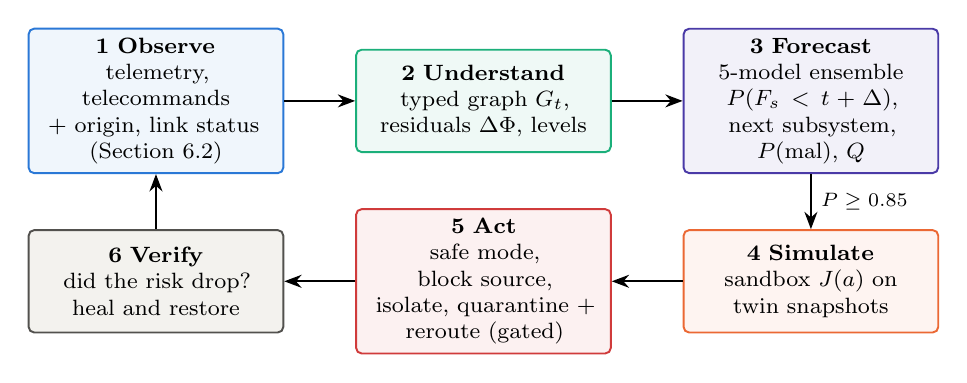
\begin{tikzpicture}[
  node distance=7mm and 9mm,
  box/.style={draw, rounded corners=2pt, align=center, font=\footnotesize, minimum height=13mm,
              text width=30mm, line width=0.7pt},
  arr/.style={-{Stealth[length=2.2mm]}, line width=0.7pt}]
\node[box, draw=cblue, fill=cblue!7] (obs) {\textbf{1 Observe}\\ telemetry, telecommands\\ + origin, link status\\ (Section 6.2)};
\node[box, draw=cgreen, fill=cgreen!7, right=of obs] (und) {\textbf{2 Understand}\\ typed graph $G_t$,\\ residuals $\Delta\Phi$, levels};
\node[box, draw=cviolet, fill=cviolet!7, right=of und] (fc) {\textbf{3 Forecast}\\ 5-model ensemble\\ $\PF$, next subsystem,\\ $P(\mathrm{mal})$, $Q$};
\node[box, draw=corange, fill=corange!7, below=of fc] (sim) {\textbf{4 Simulate}\\ sandbox $J(a)$ on\\ twin snapshots};
\node[box, draw=cred, fill=cred!7, left=of sim] (act) {\textbf{5 Act}\\ safe mode, block source,\\ isolate, quarantine +\\ reroute (gated)};
\node[box, draw=cgray, fill=clight, left=of act] (ver) {\textbf{6 Verify}\\ did the risk drop?\\ heal and restore};
\draw[arr] (obs) -- (und);
\draw[arr] (und) -- (fc);
\draw[arr] (fc) -- node[right, font=\scriptsize]{$P \geq 0.85$} (sim);
\draw[arr] (sim) -- (act);
\draw[arr] (act) -- (ver);
\draw[arr] (ver) -- (obs);
\end{tikzpicture}
\caption{CASSANDRA loop. This repository implements stages 1--3 and a reference implementation of
4--6 for closed-loop evaluation.}
\label{fig:loop}
\end{figure}

\begin{table}[H]
\centering\small
\begin{tabularx}{\linewidth}{@{}l l L@{}}
\toprule
Stage & Module & Responsibility \\
\midrule
Formats & \file{ml/schema.py} & Section 6.2 fields, forecast message, Section 6.3 episodes, \texttt{ml\_labels.json} \\
Twin stand-in & \file{ml/synthetic/} & orbital geometry, physics, attacks A1--C1, faults F1--F5, sandbox API, generator \\
Graph & \file{ml/graph.py} & node types, channels, $\Eeng$, $\Esp$ with technique IDs, ablation variants \\
Understand & \file{ml/features.py} & per-second frames, normaliser, engineering models $g_{ij}$, couplings \\
Forecast & \file{ml/model.py}, \file{ml/train.py} & temporal graph network, ensemble and ablation training \\
Calibration & \file{ml/calibration.py} & temperature scaling, reliability, ECE \\
Baselines & \file{ml/baselines.py} & static thresholds, Phase-2 trajectory forecaster, LSTM-AE, GDN \\
Online & \file{ml/online.py}, \file{ml/export.py} & messages in, forecast messages out; TorchScript, latency \\
Evaluation & \file{eval/harness.py}, \file{eval/metrics.py} & every method on every split; Section 5.8 metrics \\
Closed loop & \file{eval/closed_loop.py} & forecast, sandbox, gates, act, verify on the twin \\
Robustness & \file{eval/robustness.py} & PGD on forgeable channels \\
Datasets & \file{eval/datasets/} & checksummed downloads; CuCD-ID audit; OPS-SAT noise bank; SCAD profile; ESA-ADB \\
\bottomrule
\end{tabularx}
\caption{Implementation map.}
\label{tab:map}
\end{table}

\textbf{Rule: no ground truth in the inputs.} The forecaster reads only telemetry, telecommands
with their origin, and link status. Ground truth (\texttt{labels.json}, \texttt{ml\_labels.json},
\texttt{aurora/v1/gt/\dots}) is read only offline, by training and evaluation. Two tests protect
this:
\begin{itemize}
\item the online forecaster, fed the raw message stream, reproduces the offline features
(relative difference $2.5\times10^{-4}$);
\item a message-passing test confirms that information travels only along permitted edges.
\end{itemize}

% =====================================================================================
\section{Threat model and SPARTA anchoring}
% =====================================================================================
The adversary reaches the space segment through abused ground trust or a compromised neighbour,
but cannot falsify every independent measurement of a subsystem at once.
Table~\ref{tab:attacks} lists the episode types, which follow the attack library of the AURORA
context. SPARTA identifiers were checked against the technique pages; two of them correct the paper
(Section~\ref{sec:errata}).

\begin{table}[H]
\centering\small
\begin{tabularx}{\linewidth}{@{}l l L l@{}}
\toprule
Type & Kind & Mechanism in the generator & SPARTA \\
\midrule
A1 & attack & \texttt{HEATER} (on) with a valid ground origin, after unknown-origin pings and rejected commands, latches the heater ($+50$--$90$\,W $\times$ intensity) & IA-0009 $\rightarrow$ EX-0012 \\
A2 & attack & \texttt{SET\_MODE WHEEL\_TEST} torque bias; wheel saturates; attitude drifts & EX-0012.08 \\
A3 & attack & malicious SCIENCE/IDLE toggling; extra load $150$--$220$\,W drains the battery & EX-0012.09 \\
B1 & attack & A1 or A3 while the target channel is frozen or replays a 40\,s loop & DE-0002, EX-0001 \\
B2 & attack & A1 while a slow bias ($0.05$--$0.15$\,$^\circ$C/s) hides the temperature rise & DE-0002, DE-0003 \\
C1 & attack & compromised neighbour relays the attack over an ISL feasible at that time & IA-0003 \\
F1 & fault & slow sensor drift (temperature, SOC or attitude) & -- \\
F2 & fault & single-event upset: one corrupted sample & -- \\
F3 & fault & battery ageing: capacity $\times 0.5$--$0.7$ & -- \\
F4 & fault & natural eclipse entry & -- \\
F5 & fault & stuck heater (can reach $F$) & -- \\
N & clean & nominal operations with hard negatives & -- \\
\bottomrule
\end{tabularx}
\caption{Episode types. Hard negatives in every episode: ground passes with legitimate commands,
scheduled heater tests, relayed ISL pings and rare benign unknown-origin pings. Attacks may be
preceded by reconnaissance (pings and rejected commands): burst, sparse or none.}
\label{tab:attacks}
\end{table}

% =====================================================================================
\section{Physics-constrained cyber-physical graph}
% =====================================================================================
\subsection{Nodes and channels}
Each satellite contributes seven nodes. Six are subsystems (THERMAL, EPS, ADCS, OBC, COMMS, SUN),
and one, SAT, represents the satellite as a whole and carries its failure forecast.
Table~\ref{tab:channels} lists the 27 channels per satellite and per second. The OBC node carries
the cyber evidence: counts of telecommands by origin and type, accepted and rejected commands, and
the mode flags. All of it is derived from the telecommand and telemetry topics.

\begin{table}[H]
\centering\small
\begin{tabularx}{\linewidth}{@{}l L@{}}
\toprule
Node & Channels \\
\midrule
THERMAL & \texttt{temp\_c}, \texttt{heater\_on} \\
EPS & \texttt{soc\_pct}, \texttt{bus\_v}, \texttt{load\_w}, \texttt{solar\_w}, \texttt{current\_ma} (INA219) \\
ADCS & \texttt{att\_err\_deg}, \texttt{wheel\_rpm\_0..2}, \texttt{rate\_dps} \\
OBC & \texttt{mode\_safe}, \texttt{mode\_quarantined}, $\Delta$\texttt{cmd\_ok}, $\Delta$\texttt{cmd\_rej},
telecommands by origin (\texttt{ground}, \texttt{isl}, \texttt{unknown}) and type (\texttt{HEATER} on, \texttt{SET\_MODE}, \texttt{PING}) \\
COMMS & \texttt{ground\_contact}, \texttt{n\_isl\_peers}, \texttt{rssi\_dbm} \\
SUN & \texttt{level}, \texttt{eclipse} \\
\bottomrule
\end{tabularx}
\caption{Per-satellite channels (Section 6.2 fields plus command statistics from the telecommand topic).}
\label{tab:channels}
\end{table}

\subsection{Edge families}
\begin{itemize}
\item $\Eeng$: twelve engineering dependencies per satellite:
  \begin{itemize}
  \item OBC$\rightarrow$\{THERMAL, EPS, ADCS, COMMS\} and COMMS$\rightarrow$OBC;
  \item EPS$\leftrightarrow$THERMAL and EPS$\leftrightarrow$ADCS;
  \item SUN$\rightarrow$\{EPS, THERMAL\} and ADCS$\rightarrow$SUN.
  \end{itemize}
  Each carries a ridge-regression engineering model $g_{ij}$ fitted on nominal data.
\item $\Esp$: attack relations with technique IDs:
  \begin{itemize}
  \item COMMS$\rightarrow$OBC (IA-0009, EX-0001.01, EX-0013);
  \item OBC$\rightarrow$THERMAL (EX-0012);
  \item OBC$\rightarrow$ADCS (EX-0012.08);
  \item OBC$\rightarrow$EPS (EX-0012.09);
  \item OBC$\rightarrow$COMMS (DE-0002).
  \end{itemize}
\item Aggregation: subsystem $\rightarrow$ SAT.
\item $\Eisl(t)$: COMMS$_i \rightarrow$ COMMS$_j$ (IA-0003). These edges are present only while the
link is geometrically feasible \emph{and} enabled, so a quarantined satellite loses its links.
\item $\Elr$: learned couplings (strength $w_{ij}$, delay $\tau_{ij}$). These are attributes of
edges that $\Eeng \cup \Esp$ already permits, not new edges.
\end{itemize}
With 12 satellites, the graph has 348 directed edges. The ablation without $\Eeng$ has 264. The
unconstrained ablation, which connects every intra-satellite pair, has 564. The strongest learned
couplings are SUN$\rightarrow$EPS ($w = 0.53$) and OBC$\rightarrow$EPS ($w = 0.30$).

\subsection{Orbital geometry and ISL feasibility}
The constellation has 3 planes of 4 satellites at 550\,km and $53^\circ$ inclination, with a
$30^\circ$ phasing between planes. A ground station in Tunis has a $10^\circ$ minimum elevation.
An ISL exists when the line of sight clears the Earth by a margin of 100\,km and the range is at
most 5{,}000\,km:
\begin{equation}
\Eisl(t) = \{(i, j) \mid \mathrm{LoS}(i, j, t) = 1 \wedge d(i, j, t) \le R_{\mathrm{comm}}\}.
\end{equation}
Geometry is time-compressed by a factor of~8, so links appear and disappear within a 600\,s
episode. Subsystem physics is not compressed. Over an orbit, a satellite is in ground contact
2.3\,\% of the time and has on average 0.7 feasible ISL peers. Scenario C therefore depends
genuinely on geometry.

% =====================================================================================
\section{Data}
% =====================================================================================
\subsection{Public datasets}
Table~\ref{tab:datasets} lists the public datasets and what each one is used for.

\begin{table}[H]
\centering\small
\begin{tabularx}{\linewidth}{@{}l L L@{}}
\toprule
Dataset & Content & Use here \\
\midrule
CuCD-ID~\cite{cucd} & NOS3/cFS CCSDS telemetry: normal operation and four attack classes & audit and benchmark of a one-class cyber scorer (Section~\ref{sec:audit}) \\
OPS-SAT-AD~\cite{opssat} & 2{,}123 labelled ESA OPS-SAT telemetry segments & nominal test segments become a bank of real residual noise and gaps for the \texttt{test\_real} split \\
SCAD~\cite{scad} & simulated reaction-wheel override attacks with matched baselines & measured propagation profile (Section~\ref{sec:scad}) \\
ESA-ADB~\cite{esaadb} & operational telemetry benchmark & loader written; not evaluated (3.7--4.1\,GB per mission) \\
\bottomrule
\end{tabularx}
\caption{Public datasets. Downloads are checksummed (SHA-256 for CuCD-ID, MD5 for OPS-SAT-AD); nothing is committed.}
\label{tab:datasets}
\end{table}

\subsection{CuCD-ID audit: a session shortcut and a temporal drift}\label{sec:audit}
Each CuCD-ID class was recorded in its own session, and some columns are constant within a
session. With a time-based split, a classifier reaches \rCucdShortcut\,\% accuracy on the memory
columns alone, and \rCucdTraffic\,\% on traffic columns. With one session per class, class and
session are confounded, so near-perfect supervised accuracy on this dataset says nothing about
attack detection and should not be reported. We use traffic-behaviour features, a time split per
class and a one-class detector
fitted on normal traffic only. On attack types it has never seen (leave-one-attack-out), this
detector reaches an AUROC of \rCucdLoaoMin--\rCucdLoaoMax. Normal traffic also drifts:
\rCucdDrift\,\% of later normal rows exceed the 0.95 score quantile of earlier ones. A deployed
cyber scorer therefore needs online recalibration.

\subsection{SCAD: measured attack propagation}\label{sec:scad}
SCAD provides attack runs and baseline runs of the same scenario. For each of \rScadRuns{} attack
runs, we compare every subsystem with its matched baseline and record whether, and when, it
departs. The wheels and torque rods are affected immediately. Attitude follows in half of the runs.
Power departs in \rScadPowerFrac\,\% of runs, a median \rScadPowerDelay\,s after the override, and
the star tracker in \rScadStarTrackerFrac\,\%, a median \rScadStarTrackerDelay\,s after it
(Fig.~\ref{fig:scad}). These measured delays support the propagation structure of the graph.
However, only \rScadReachF\,\% of the attack runs lose more than \rScadPointing$^\circ$ of pointing
relative to the baseline, which is the attitude clause of $F$. SCAD is therefore a detection and
propagation benchmark, not a time-to-failure benchmark, and we do not report lead time on it.

\begin{figure}[H]
\centering
\maybefig{fig_scad_cascade}{0.75\linewidth}
\caption{SCAD: fraction of attack runs in which each subsystem departs from its matched baseline,
with the median delay after the override.}
\label{fig:scad}
\end{figure}

\subsection{Synthetic constellation (stand-in for twin v1)}
No public dataset contains attacks that propagate to a physical failure on a constellation. The
synthetic twin (\file{ml/synthetic/}) therefore generates them in the AURORA formats. Its physics
runs at 1\,Hz.
\begin{itemize}
\item \textbf{Thermal.} $C\,\dot T = P_{\mathrm{heater}} + P_{\mathrm{sun}}(1-\mathrm{ecl}) +
P_{\mathrm{int}} + P_{\mathrm{sci}} - G\,(T - T_{\mathrm{env}})$, with a thermostat between 5 and
9\,$^\circ$C. Attack heater power is added on top.
\item \textbf{EPS.} $E\,\dot{\mathrm{SOC}} = P_{\mathrm{solar}} - P_{\mathrm{load}}$, with
$P_{\mathrm{solar}} = P_{\mathrm{panel}} \cos\theta_{\mathrm{err}} (1-\mathrm{ecl})$. The load
includes heater, science, transmitter and wheel power. Bus voltage and current follow from the load.
\item \textbf{ADCS.} The wheels relax to their reference. A torque bias accelerates one wheel to
saturation, after which attitude drifts. Ground passes add benign slews of 2--6$^\circ$.
\item \textbf{Commands.} Commands are executed by the OBC with their origin. Health pings, science
windows and heater tests follow a plan. Malicious and relayed commands are delivered with
ISL-feasibility checks.
\item \textbf{Reported telemetry.} Reported values are the true state plus noise from a generator
family (Gaussian, AR(1) or Student-$t$, or real OPS-SAT residuals with gaps), with masking applied
for B1 and B2.
\end{itemize}
\textbf{Exact labels.} After each episode the twin replays the same episode without the anomaly,
using the same noise and an attack random stream separate from the plan's. The first time each
subsystem departs from this counterfactual is its \texttt{affected\_t}. A test asserts that no
subsystem is affected before onset, and that clean episodes never reach $F$. The sandbox API
(\texttt{snapshot}, \texttt{restore}, \texttt{apply}, \texttt{step}) is the one the closed loop uses.

\subsection{Splits}
Splits are made by whole episode, with a separate seed per split (Table~\ref{tab:splits}).
Training uses the drift shapes \{ramp, saturating\}, the noise models \{Gaussian, AR(1)\} and
intensities 0.7--1.0. Every \texttt{test\_ood} episode has at least one held-out knob: pulsed drift,
Student-$t$ noise or intensity 0.5--0.7. \texttt{test\_real} replaces generator noise with OPS-SAT
residuals and gaps, and over-samples clean and fault episodes.

\begin{table}[H]
\centering\small
\begin{tabular}{@{}lrrrrrrr@{}}
\toprule
Split & Episodes & A & B & C & F & N & Failing satellites \\
\midrule
train & 800 & 224 & 104 & 104 & 221 & 147 & 545 \\
val & 200 & 45 & 32 & 27 & 56 & 40 & 136 \\
test\_id & 300 & 92 & 38 & 37 & 92 & 41 & 205 \\
test\_ood & 300 & 81 & 40 & 42 & 75 & 62 & 113 \\
test\_real & 200 & 33 & 32 & 0 & 69 & 66 & 69 \\
\bottomrule
\end{tabular}
\caption{Episode splits (600\,s episodes, 12 satellites). Failing satellites reach $F$ when no
response is applied.}
\label{tab:splits}
\end{table}

\subsection{Targets}
For a window ending at $t$ and a satellite with critical tick $c$, the targets are:
\begin{itemize}
\item \textbf{Hazard.} $y_\Delta = \mathbb{1}[t < c \le t + \Delta]$ for
$\Delta \in \{10, 30, 60, 120\}$\,s. The target is masked after failure. It is
\emph{right-censored} when the satellite is at risk but the episode ends before $t + \Delta$
without failing.
\item \textbf{Next subsystem.} The next subsystem whose \texttt{affected\_t} lies after $t$.
\item \textbf{Malicious.} 1 for attacks and 0 for faults.
\end{itemize}
The next-subsystem and malicious targets are defined once the anomaly has started.

% =====================================================================================
\section{Understand stage}
% =====================================================================================
\textbf{Normalisation and differences.} Each channel is normalised with the mean and standard
deviation of the benign training episodes, and its first difference is normalised separately.

\textbf{Engineering models and residuals.} For every engineering edge $(i, j)$, two ridge
regressions are fitted on nominal data:
\begin{itemize}
\item $g_{ij}$ predicts the change of node $j$'s channels from node $i$'s previous state;
\item $h_{ij}$ predicts node $j$'s level from node $i$'s current state.
\end{itemize}
From them the engine computes two residuals:
\begin{equation}
\Delta\Phi_{ij,t} = \big\lVert (x_{j,t} - x_{j,t-1}) - g_{ij}(x_{i,t-1}) \big\rVert,\qquad
\ell_{ij,t} = \big\lVert x_{j,t} - h_{ij}(x_{i,t}) \big\rVert.
\end{equation}
$\Delta\Phi$ separates changes that the engineering model explains, such as an eclipse or a pass,
from induced ones. $\ell$ captures cross-domain consistency. A frozen temperature next to a rising
heater load, or a stable SOC next to a rising bus current, produces a large $\ell$ on the edge that
links them.

\textbf{Learned couplings.} The activity of a subsystem is the RMS of its normalised first
differences. On every pair permitted by $\Eeng \cup \Esp$, the strength $w_{ij} \in [0, 1]$ is the
maximum normalised cross-correlation between the activities of $i$ and $j$ over the delays
0--15\,s, and $\tau_{ij}$ is the delay at which it peaks. Both are computed on the training attack
episodes, which are where propagation happens.

All of these are computed \emph{inside} the forecaster module from the raw frames. Training,
online inference, TorchScript export and the PGD adversary therefore use the same code path.

% =====================================================================================
\section{Temporal graph forecaster}
% =====================================================================================
\subsection{Architecture}
The input is a 30\,s window of per-satellite frames $[W, S, 27]$ and the current ISL state (66
pairs).
\begin{enumerate}
\item \textbf{Node encoders.} Each node takes its normalised channels and their first
differences. A projection specific to its node type and a type embedding feed a GRU over the
window, whose final state is the node's temporal memory $h_i$.
\item \textbf{Edge features.} A small GRU over the sequence $(\Delta\Phi_{ij}, \ell_{ij})$ of
each engineering edge gives a dynamic edge state. It is concatenated with the edge-family flags and
the learned coupling $(w_{ij}, \tau_{ij})$ to form $e_{ij}$.
\item \textbf{Message passing.} Three rounds of relation-aware attention:
\begin{align}
m_{ji} &= \mathrm{MLP}\big([h_j;\, h_i;\, e_{ji}]\big) + W_{r(ji)}\, h_j, \\
h_i &\leftarrow \mathrm{LayerNorm}\Big(h_i + \mathrm{ReLU}\Big(\textstyle\sum_{j \in \mathcal{N}_t(i)} \alpha_{ji}\, m_{ji}\Big)\Big),
\end{align}
with one weight matrix per relation $r \in \{\mathrm{eng}, \mathrm{SPARTA}, \mathrm{agg},
\mathrm{ISL}\}$, as in R-GCN~\cite{rgcn}. The attention $\alpha_{ji}$, computed from
$[h_j; h_i; e_{ji}]$, is normalised over the incoming edges present at $t$, as in GAT~\cite{gat}.
ISL edges are masked by the live link state. Three rounds reach COMMS$_i \rightarrow$ COMMS$_j
\rightarrow$ OBC$_j \rightarrow$ THERMAL$_j$.
\item \textbf{Hazard head.} The head reads each satellite's SAT node together with the mean and
the maximum of its subsystem nodes. Discrete-time hazards $\lambda_k = \sigma(b_k)$ for the bins
$(0, 10], (10, 30], (30, 60], (60, 120]$\,s give
\begin{equation}
P(F_s < t + \Delta_k) = 1 - \prod_{j \le k} (1 - \lambda_j),
\end{equation}
which is monotone in the horizon by construction.
\item \textbf{Other heads.} For the next affected subsystem, each subsystem node gets a score and a
softmax is taken over the six. $P(\mathrm{malicious} \mid \mathrm{anomaly})$ is a sigmoid on the
same satellite summary as the hazard head.
\end{enumerate}
Each model has 42.7k parameters (hidden size 32, edge hidden size 16).

\subsection{Training}
\begin{itemize}
\item \textbf{Loss.} Binary cross-entropy on the hazard bins with positive weight 3 and the
censoring mask, plus $0.3\times$ cross-entropy on the next subsystem and $0.3\times$ binary
cross-entropy on malicious.
\item \textbf{Windows.} Eight windows per episode and epoch: half uniform, half from 30\,s before
onset to just after the last failure.
\item \textbf{Optimisation.} Adam with learning rate $2\times10^{-3}$, batch 48, at most 8 epochs,
and early stopping on validation loss (patience 3).
\item \textbf{Models.} Five seeds form the ensemble. The three ablations use seed~0.
\end{itemize}

\subsection{Calibration and uncertainty}
A single temperature is fitted on validation windows to the ensemble-mean hazard logits
(Guo et al.~\cite{guo}). Expected calibration error uses 10 equal-width bins per horizon.

The uncertainty of the response engine is the \emph{standard deviation} of $P(F_s < t+60\,\mathrm{s})$
across the five members~\cite{ensembles}. A variance of a probability is at most 0.25, so a
variance could never exceed the gate $\theta_{\mathrm{uncert}} = 0.35$ (erratum~3).

% =====================================================================================
\section{Response engine (reference implementation)}
% =====================================================================================
When $P(F_s < t+60\,\mathrm{s}) \ge 0.85$, the sandbox snapshots the twin and, for each candidate
action, restores the snapshot, applies the action and rolls the twin forward 30\,s with the
forecaster in the loop. It then scores
\begin{equation}
J(a) = w_r R(a) + w_m\,[1 - U(a)] + w_c C(a) + w_q Q(a),\qquad (w_r, w_m, w_c, w_q) = (1, 0.5, 0.3, 0.5),
\end{equation}
where:
\begin{itemize}
\item $R$ is the highest forecast $P(F < t+60\,\mathrm{s})$ over the constellation at the end of
the rollout, so an action that pushes risk onto a neighbour is penalised;
\item $U$ is the fraction of satellites still in nominal mode;
\item $C$ is a fixed cost per action;
\item $Q$ is the ensemble standard deviation for the target satellite.
\end{itemize}
The candidate actions and their SPARTA countermeasures are:
\begin{itemize}
\item \texttt{none};
\item \texttt{safe\_mode} (CM0042);
\item \texttt{block\_source} (CM0032), which blocks the unknown and ISL origins seen on the
satellite in the last 120\,s and drops their queued commands;
\item \texttt{isolate\_subsystem} (CM0042), which isolates the heater and sets IDLE mode;
\item \texttt{quarantine\_reroute} (CM0070), which sets QUARANTINED mode and disables the
satellite's ISLs in both directions so traffic reroutes around it.
\end{itemize}

Two gates prevent self-denial of service:
\begin{itemize}
\item \textbf{Uncertainty gate.} If the chosen action has $Q > 0.35$, the engine does not execute
it and puts the satellite in safe mode (a safe hold for ground review).
\item \textbf{Isolation budget.} \texttt{quarantine\_reroute} is offered only while quarantines in
the current orbital period stay within 25\,\% of the constellation.
\end{itemize}
A satellite is planned at most every 10\,s. A contained satellite is restored once its forecast
has stayed below the flag threshold (0.30) for 10 consecutive steps. The sandbox uses the
simulator as its state-transition model, so closed-loop results are an upper bound for an
engineering-model twin.

% =====================================================================================
\section{Evaluation protocol}
% =====================================================================================
\begin{itemize}
\item \textbf{Matched false-positive rate.} For each method, $\tau$ is the 99.9\,\% quantile of
its scores on \emph{validation benign timesteps}: every tick of the satellites in clean and fault
episodes that never reach $F$. $\tau$ is applied unchanged to the test splits, and the realised FPR
and the false alarms per satellite-hour are reported. Fixing $\tau$ on validation data, rather than
on each test split, is what a deployment would do. It also shows which methods hold their
false-alarm rate under distribution shift.
\item \textbf{Lead time.} $T_{\mathrm{alert}}$ is the first tick at or after the episode's onset
with score $\ge \tau$, and $T_{\mathrm{lead}} = T_{\mathrm{critical}} - T_{\mathrm{alert}}$. An
alert at or after $T_{\mathrm{critical}}$ is a miss. We report the recall of failing satellites,
the median lead and its IQR over detected satellites, and 95\,\% bootstrap intervals over episodes.
\item \textbf{Action threshold.} The same quantities at the response engine's action threshold
($P \ge 0.85$, \texttt{ensemble@act}): how early the system would \emph{act}, not only warn.
\item \textbf{Other metrics.}
  \begin{itemize}
  \item episode-level precision and recall;
  \item AUROC and AUPRC of $P(F_s < t+60\,\mathrm{s})$ on satellite-ticks with a defined target;
  \item ECE per horizon;
  \item next-subsystem top-1 and top-3;
  \item malicious-vs-fault AUROC;
  \item breakdowns by episode type, scenario and precursor.
  \end{itemize}
\item \textbf{Ticks.} Models are evaluated every 6\,s everywhere, an unbiased sample for FPR, and
every 2\,s from onset to the last failure, where lead time is measured. Ground truth only
schedules evaluation; it never enters the inputs.
\item \textbf{Baselines.} The baselines are:
  \begin{itemize}
  \item static thresholds on the three critical channels, scored by proximity to the limit;
  \item the Phase-2 trajectory forecaster (8-sample slope, $\hat P = \mathrm{clip}(1 - t_c/H)$);
  \item an LSTM autoencoder~\cite{lstmae};
  \item GDN~\cite{gdn}, with per-sensor embeddings, a learned top-$k$ graph and robustly
  normalised forecast errors.
  \end{itemize}
  The LSTM autoencoder and GDN are trained on clean training episodes.
\end{itemize}

% =====================================================================================
\section{Results (simulation)}\label{sec:results}
% =====================================================================================
Every measured number in this section is a macro produced by \file{eval/paper_numbers.py} from
\file{results/}. Settings, such as the number of PGD steps, are stated as configured. The results
come from synthetic episodes; Section~\ref{sec:limits} lists what this does and does not show.

\subsection{Main result}
\begin{table}[H]
\centering\small
\setlength{\tabcolsep}{4pt}
\begin{tabular}{@{}lcccccc@{}}
\toprule
 & \multicolumn{2}{c}{In-distribution} & \multicolumn{2}{c}{Held-out families} & \multicolumn{2}{c}{OPS-SAT noise} \\
\cmidrule(lr){2-3}\cmidrule(lr){4-5}\cmidrule(l){6-7}
Method & Lead (s) & Recall & Lead (s) & Recall & Lead (s) & Recall \\
\midrule
\textbf{CASSANDRA, 5-model ensemble} & \textbf{\rEnsIDLead} & \textbf{\rEnsIDRec} & \textbf{\rEnsOODLead} & \textbf{\rEnsOODRec} & \textbf{\rEnsRealLead} & \textbf{\rEnsRealRec} \\
\quad 95\,\% CI of the median & \multicolumn{2}{c}{\rEnsIDLeadLo--\rEnsIDLeadHi} & \multicolumn{2}{c}{\rEnsOODLeadLo--\rEnsOODLeadHi} & \multicolumn{2}{c}{\rEnsRealLeadLo--\rEnsRealLeadHi} \\
Single model & \rSingleIDLead & \rSingleIDRec & \rSingleOODLead & \rSingleOODRec & \rSingleRealLead & \rSingleRealRec \\
GDN & \rGdnIDLead & \rGdnIDRec & \rGdnOODLead & \rGdnOODRec & \rGdnRealLead & \rGdnRealRec \\
LSTM autoencoder & \rAeIDLead & \rAeIDRec & \rAeOODLead & \rAeOODRec & \rAeRealLead & \rAeRealRec \\
Phase-2 trajectory & \rTrajIDLead & \rTrajIDRec & \rTrajOODLead & \rTrajOODRec & \rTrajRealLead & \rTrajRealRec \\
Static thresholds & \rThrIDLead & \rThrIDRec & \rThrOODLead & \rThrOODRec & \rThrRealLead & \rThrRealRec \\
\midrule
Failing satellites & \multicolumn{2}{c}{\rNfailID} & \multicolumn{2}{c}{\rNfailOOD} & \multicolumn{2}{c}{\rNfailReal} \\
\bottomrule
\end{tabular}
\caption{Median warning lead time before the critical state and recall of failing satellites, with
every method's threshold set at 0.1\,\% FPR on validation benign timesteps.}
\label{tab:main}
\end{table}

\begin{table}[H]
\centering\small
\setlength{\tabcolsep}{4pt}
\begin{tabular}{@{}lcccccc@{}}
\toprule
Method & AUROC & AUPRC & FPR ID (\%) & FPR OOD (\%) & FPR real (\%) & Alarms / sat-h (ID) \\
\midrule
CASSANDRA & \rEnsIDAuroc & \rEnsIDAuprc & \rEnsIDVfpr & \rEnsOODVfpr & \rEnsRealVfpr & \rEnsIDFah \\
GDN & \rGdnIDAuroc & \rGdnIDAuprc & \rGdnIDVfpr & \rGdnOODVfpr & \rGdnRealVfpr & \rGdnIDFah \\
LSTM autoencoder & \rAeIDAuroc & \rAeIDAuprc & \rAeIDVfpr & \rAeOODVfpr & \rAeRealVfpr & \rAeIDFah \\
Phase-2 trajectory & \rTrajIDAuroc & \rTrajIDAuprc & \rTrajIDVfpr & \rTrajOODVfpr & \rTrajRealVfpr & \rTrajIDFah \\
Static thresholds & \rThrIDAuroc & \rThrIDAuprc & \rThrIDVfpr & \rThrOODVfpr & \rThrRealVfpr & \rThrIDFah \\
\bottomrule
\end{tabular}
\caption{Ranking quality of the 60\,s forecast on the in-distribution split, and false-alarm
behaviour with thresholds fixed on validation data (target 0.10\,\%).}
\label{tab:fpr}
\end{table}

\begin{figure}[H]
\centering
\maybefig{fig_lead_time}{\linewidth}
\caption{Mean lead time (misses count as 0) and recall for every method on the three test splits.}
\label{fig:lead}
\end{figure}

\textbf{Reading.} With every threshold fixed on validation data, the ensemble detects every failing
satellite on all three test splits. The lead is a median \rEnsIDLead\,s in distribution (95\,\% CI
\rEnsIDLeadLo--\rEnsIDLeadHi), \rEnsOODLead\,s on held-out families and \rEnsRealLead\,s under
OPS-SAT noise. The realised false-positive rates on test benign steps are \rEnsIDVfpr,
\rEnsOODVfpr{} and \rEnsRealVfpr\,\%. Two of them are above the 0.10\,\% target fixed on validation
data, which is the expected cost of a threshold that is not re-tuned on test data.

The baselines fall into two groups:
\begin{itemize}
\item \textbf{Static thresholds and the trajectory forecaster} (recall \rThrIDRec{} and
\rTrajIDRec{} in distribution) warn late: \rThrIDLead{} and \rTrajIDLead\,s. Their recall falls to
\rThrRealRec{} and \rTrajRealRec{} on the real-noise split. The cause is the split's composition,
not the noise: on unmasked heater latches they keep recall \rThrRealScenARec{} and
\rTrajRealScenARec. The losses come from masked failures, which make up \rMaskShareReal\,\% of
that split's failing satellites, against \rMaskShareID\,\% in distribution.
\item \textbf{GDN and the LSTM autoencoder} warn early when they fire, but miss many failures
(recall \rGdnIDRec{} and \rAeIDRec). GDN fires in short bursts: \rGdnIDFah{} alarm events per
satellite-hour, against \rEnsIDFah{} for the ensemble.
\end{itemize}

At the matched rate, the alert threshold on $P(F < t+60\,\mathrm{s})$ is \rEnsIDThresh, and the
alert comes a median \rEnsIDDelay\,s after the satellite's first anomalous activity. Lead time
measured this way is therefore mostly \emph{time from detection to failure}, which can exceed the
horizon. The operating point that matters for action is $P \ge 0.85$
(Section~\ref{sec:heads}).

\subsection{By episode type, scenario and precursor}
\begin{table}[H]
\centering\small
\begin{tabular}{@{}lccc@{}}
\toprule
Type & Failing satellites & Recall & Median lead (s) \\
\midrule
A1 heater latch & \rEnsIDTypeAOneN & \rEnsIDTypeAOneRec & \rEnsIDTypeAOneLead \\
A2 wheel torque bias & \rEnsIDTypeATwoN & \rEnsIDTypeATwoRec & \rEnsIDTypeATwoLead \\
A3 power drain & \rEnsIDTypeAThreeN & \rEnsIDTypeAThreeRec & \rEnsIDTypeAThreeLead \\
B1 freeze / replay & \rEnsIDTypeBOneN & \rEnsIDTypeBOneRec & \rEnsIDTypeBOneLead \\
B2 slow bias & \rEnsIDTypeBTwoN & \rEnsIDTypeBTwoRec & \rEnsIDTypeBTwoLead \\
C1 ISL propagation & \rEnsIDTypeCOneN & \rEnsIDTypeCOneRec & \rEnsIDTypeCOneLead \\
F5 stuck heater (fault) & \rEnsIDTypeFFiveN & \rEnsIDTypeFFiveRec & \rEnsIDTypeFFiveLead \\
\bottomrule
\end{tabular}
\caption{CASSANDRA ensemble on \texttt{test\_id} by episode type.}
\label{tab:types}
\end{table}

\begin{table}[H]
\centering\small
\begin{tabular}{@{}lcccccc@{}}
\toprule
 & \multicolumn{2}{c}{Masking (B)} & \multicolumn{2}{c}{Propagation (C)} & \multicolumn{2}{c}{No precursor$^{a}$} \\
\cmidrule(lr){2-3}\cmidrule(lr){4-5}\cmidrule(l){6-7}
Method & Lead (s) & Recall & Lead (s) & Recall & Lead (s) & Recall \\
\midrule
CASSANDRA & \rEnsIDScenBLead & \rEnsIDScenBRec & \rEnsIDScenCLead & \rEnsIDScenCRec & \rEnsIDPreNoneLead & \rEnsIDPreNoneRec \\
GDN & \rGdnIDScenBLead & \rGdnIDScenBRec & \rGdnIDScenCLead & \rGdnIDScenCRec & \rGdnIDPreNoneLead & \rGdnIDPreNoneRec \\
LSTM autoencoder & \rAeIDScenBLead & \rAeIDScenBRec & \rAeIDScenCLead & \rAeIDScenCRec & \rAeIDPreNoneLead & \rAeIDPreNoneRec \\
Phase-2 trajectory & \rTrajIDScenBLead & \rTrajIDScenBRec & \rTrajIDScenCLead & \rTrajIDScenCRec & \rTrajIDPreNoneLead & \rTrajIDPreNoneRec \\
Static thresholds & \rThrIDScenBLead & \rThrIDScenBRec & \rThrIDScenCLead & \rThrIDScenCRec & \rThrIDPreNoneLead & \rThrIDPreNoneRec \\
\bottomrule
\end{tabular}
\caption{The hard cases on \texttt{test\_id}: masked telemetry, cross-satellite propagation, and
failing satellites without a reconnaissance precursor. $^{a}$This group also includes the
stuck-heater faults (F5), which never have a precursor. A dash means nothing was detected, so the
median lead is undefined.}
\label{tab:hard}
\end{table}

\begin{figure}[H]
\centering
\maybefig{fig_example_masking}{0.8\linewidth}
\caption{A masked-telemetry episode (B1) from \texttt{test\_id}. Top: reported channels; the
temperature stays frozen while the bus current reveals the latched heater. Bottom: the forecast at
four horizons. The vertical lines mark onset and the critical time, and the dotted line marks
$\tau$. The alert fires \rFigAlertDelay\,s after onset, but the forecast falls below 0.5
\rFigFallBefore\,s before the failure, when the load changes. This failure mode matters for a
response engine that waits.}
\label{fig:masking}
\end{figure}

\textbf{Reading.} Masking separates the methods most clearly. Static thresholds catch
\rThrIDScenBRec{} of masked failures and the trajectory forecaster \rTrajIDScenBRec, because both
read the forged channel. The ensemble catches \rEnsIDScenBRec, a median \rEnsIDScenBLead\,s ahead.
Only the temperature or state of charge is forged, while the heater state and the bus current stay
honest. The ablations without $\Eeng$ (\rNoEngIDScenBRec) and without residuals
(\rNoResIDScenBRec) catch masking just as well, so on this benchmark the evidence appears to be the
honest channels themselves, not the engineering edges. An ablation that hides those channels too
would test this.

For cross-satellite propagation (C1), thresholds detect every victim, but only \rThrIDScenCLead\,s
ahead, against \rEnsIDScenCLead\,s for the ensemble.

The precursor groups mix attacks and faults: the ``none'' group includes the stuck-heater faults.
We therefore do not compare them; the stress test below addresses the role of the command
evidence directly.

\subsection{Ablations}
\begin{table}[H]
\centering\small
\begin{tabular}{@{}lccccc@{}}
\toprule
Variant & Lead ID (s) & Recall ID & AUROC ID & Lead real (s) & FPR real (\%) \\
\midrule
Full (5-model ensemble) & \rEnsIDLead & \rEnsIDRec & \rEnsIDAuroc & \rEnsRealLead & \rEnsRealVfpr \\
Single model & \rSingleIDLead & \rSingleIDRec & \rSingleIDAuroc & \rSingleRealLead & \rSingleRealVfpr \\
Without $\Eeng$ & \rNoEngIDLead & \rNoEngIDRec & \rNoEngIDAuroc & \rNoEngRealLead & \rNoEngRealVfpr \\
Unconstrained edges & \rUnconIDLead & \rUnconIDRec & \rUnconIDAuroc & \rUnconRealLead & \rUnconRealVfpr \\
Without residuals & \rNoResIDLead & \rNoResIDRec & \rNoResIDAuroc & \rNoResRealLead & \rNoResRealVfpr \\
\bottomrule
\end{tabular}
\caption{Ablations at the same 0.1\,\% validation FPR.}
\label{tab:ablation}
\end{table}

\textbf{Reading: a partly negative result, reported as such.} Every variant detects every failing
satellite, and its median lead lies inside the confidence interval of the full model. The
false-positive rates differ by at most a few hundredths of a percentage point; no interval was
computed for them. The ensemble improves ranking over a single model (AUPRC \rEnsIDAuprc{} vs.\
\rSingleIDAuprc).

The training loss does separate the variants:
\begin{itemize}
\item the five full models reach a best validation loss of \rValFullMin--\rValFullMax;
\item without $\Eeng$, \rValNoEng: a clearly worse fit;
\item unconstrained edges, \rValUncon;
\item without residuals, \rValNoRes, lower than every full model.
\end{itemize}
The detection metrics saturate, because an attack's actuation appears in housekeeping telemetry
within seconds (Section~\ref{sec:limits}). They therefore cannot show whether the better fit with
$\Eeng$ turns into earlier or more reliable warnings. Testing these design choices requires
stealthier actuation and twin or hardware episodes, not more of the same data. This is the first
item of the roadmap.

\subsection{Horizons, action threshold, calibration and the other heads}\label{sec:heads}
\begin{table}[H]
\centering\small
\begin{tabular}{@{}lcccc@{}}
\toprule
Horizon $\Delta$ & 10\,s & 30\,s & 60\,s & 120\,s \\
\midrule
Median lead at matched FPR, ID (s) & \rEnsHTenIDLead & \rEnsHThirtyIDLead & \rEnsHSixtyIDLead & \rEnsHTwoMinIDLead \\
Recall, ID & \rEnsHTenIDRec & \rEnsHThirtyIDRec & \rEnsHSixtyIDRec & \rEnsHTwoMinIDRec \\
ECE in distribution & \rEceIDTen & \rEceIDThirty & \rEceIDSixty & \rEceIDTwoMin \\
ECE held-out families & \rEceOODTen & \rEceOODThirty & \rEceOODSixty & \rEceOODTwoMin \\
ECE OPS-SAT noise & \rEceRealTen & \rEceRealThirty & \rEceRealSixty & \rEceRealTwoMin \\
\bottomrule
\end{tabular}
\caption{Per-horizon behaviour (temperature $T = \rTemp$).}
\label{tab:horizons}
\end{table}

\begin{itemize}
\item \textbf{Action threshold.} At $P \ge 0.85$, the ensemble flags \rActIDRec{} of the failing
satellites a median \rActIDLead\,s before the critical state (held-out families: \rActOODRec,
\rActOODLead\,s; OPS-SAT noise: \rActRealRec, \rActRealLead\,s). The realised FPR on benign steps is
\rActIDVfpr\,\% in distribution.
\item \textbf{Next affected subsystem.} Top-1 accuracy is \rNextIDTop\,\% and top-3 accuracy is
\rNextIDTopThree\,\% in distribution (held-out families: \rNextOODTop\,\% and \rNextOODTopThree\,\%).
\item \textbf{Malicious vs fault.} The AUROC is \rMalIDAuroc{} in distribution, \rMalOODAuroc{} on
held-out families and \rMalRealAuroc{} under OPS-SAT noise.
\item \textbf{Uncertainty.} The ensemble standard deviation exceeds the 0.35 gate on \rQgateID\,\%
of in-distribution steps, \rQgateOOD\,\% of held-out-family steps and \rQgateReal\,\% of real-noise
steps.
\end{itemize}

\begin{figure}[H]
\centering
\maybefig{fig_calibration}{0.5\linewidth}
\caption{Expected calibration error of $P(F_s < t+\Delta)$ by horizon and split.}
\label{fig:calibration}
\end{figure}

\textbf{Reading.}
\begin{itemize}
\item \textbf{Calibration.} ECE is very low on every split. Most steps are confidently negative,
however, so the aggregate ECE says little about the high-risk range. A reliability diagram
restricted to at-risk satellites is the honest next check.
\item \textbf{Action threshold.} Recall at $P \ge 0.85$ drops from \rActIDRec{} in distribution to
\rActOODRec{} on held-out families and \rActRealRec{} under real noise. The forecast is
conservative under shift: it still warns at the matched rate, but less often reaches the action
level before the failure.
\item \textbf{Next subsystem.} The head holds on held-out families but drops to \rNextRealTop\,\%
top-1 on the real-noise split. That split also contains only heater-latch and masked attacks, so
the result files cannot separate the effect of noise from the different attack mix.
\item \textbf{Uncertainty.} The gate is reached on \rQgateOOD\,\% of held-out-family steps, against
\rQgateID\,\% in distribution: it rises under shift but stays rare.
\end{itemize}

\subsection{Closed loop}
We re-ran \rClEp{} test episodes (\rClAtt{} attacks; \rClNom{} clean or fault) on the twin with
CASSANDRA acting. Without a response, \rClFailWithout{} satellites reach $F$. With the response,
\rClAverted{} of them are averted (\rClAvertedPct\,\%) and \rClNewFail{} new failures occur. The
loop made \rClFalse{} false containments of satellites that were not at risk, which is
\rClFalsePerOrbit{} per orbit. The mean availability of the constellation was \rClAvail\,\%. Of
the \rClDecisions{} actions, \rClSafe{} were safe mode, \rClBlock{} blocked a source, \rClIso{}
isolated a subsystem and \rClReroute{} quarantined and rerouted. \rClGated{} decisions were held by
the uncertainty gate. A counterfactual plan takes \rLatPlan\,ms (median; p95 \rLatPlanP\,ms) on an
x86 laptop.

\begin{table}[H]
\centering\small
\begin{tabular}{@{}lcccccccc@{}}
\toprule
Type & A1 & A2 & A3 & B1 & B2 & C1 & F5 & Total \\
\midrule
Failing without response & \rClFailAOne & \rClFailATwo & \rClFailAThree & \rClFailBOne & \rClFailBTwo & \rClFailCOne & \rClFailFFive & \rClFailWithout \\
Averted by CASSANDRA & \rClAvertAOne & \rClAvertATwo & \rClAvertAThree & \rClAvertBOne & \rClAvertBTwo & \rClAvertCOne & \rClAvertFFive & \rClAverted \\
\bottomrule
\end{tabular}
\caption{Closed loop by episode type (\texttt{test\_id}, simulation).}
\label{tab:closedloop}
\end{table}

\textbf{Reading.}
\begin{itemize}
\item \textbf{What works.} Heater latches, wheel attacks and the stuck heater were averted, with
no false containment and no new failure.
\item \textbf{What did not.}
  \begin{itemize}
  \item \textbf{Battery drains (A3).} The loop acted on every drain (safe mode), yet the battery
  still reached its limit, so the action came too late or was the wrong one.
  \item \textbf{Propagated failures (C1).} The forecast did cross the action threshold, but in the
  propagation episodes \rClNoneCOne{} planner calls chose \emph{no action}: the trade-off in $J(a)$
  favoured availability over residual risk.
  \item \textbf{Replay or freeze masking (B1).} \rClAvertBOne{} of \rClFailBOne{} failures were
  averted.
  \end{itemize}
  The next steps are acting earlier (on the 60\,s forecast before it reaches 0.85), adding
  load-shedding actions, and re-weighting $J(a)$ when a neighbour is compromised. The per-decision
  tables are in \file{results/eval/closed_loop.json}.
\item \textbf{Planning time.} A plan takes a median \rLatPlan\,ms, \rLatPlanRatio{} times the
150\,ms budget, and varied from \rLatPlanMin{} to \rLatPlanMax\,ms over \rClPlans{} plans with
machine load. The in-loop forecast step (eager mode) took a median \rClStepMs\,ms. The sandbox rolls
the full twin and the five-model forecaster forward 30\,s for each of five actions; on board this
must become a light engineering-model rollout.
\end{itemize}

\subsection{Adversarial robustness}
A PGD adversary (8 steps) perturbs every forgeable housekeeping channel (THERMAL, EPS and ADCS,
except \texttt{heater\_on}) of every satellite, within $\pm\varepsilon$ nominal standard deviations,
over the whole window. Its goal is to suppress the failing satellite's $P(F_s < t+60\,\mathrm{s})$
on \rRobN{} attacked satellites. Telecommands, the sun sensor
and link status are not forgeable, because they arrive from other paths.

\begin{table}[H]
\centering\small
\begin{tabular}{@{}lcccc@{}}
\toprule
$\varepsilon$ (nominal std) & 0 & 0.25 & 0.5 & 1 \\
\midrule
CASSANDRA recall & \rRobZeroRec & \rRobARec & \rRobBRec & \rRobCRec \\
CASSANDRA median lead (s) & \rRobZeroLead & \rRobALead & \rRobBLead & \rRobCLead \\
Mean ensemble std $Q$ & \rRobZeroQ & \rRobAQ & \rRobBQ & \rRobCQ \\
Static thresholds recall & \rRobZeroThrRec & \rRobAThrRec & \rRobBThrRec & \rRobCThrRec \\
Static thresholds median lead (s) & \rRobZeroThrLead & \rRobAThrLead & \rRobBThrLead & \rRobCThrLead \\
\bottomrule
\end{tabular}
\caption{PGD on forgeable channels (CASSANDRA rows). The static-threshold rows are not PGD: the
same budget is applied as a fixed shift of the critical channels away from their limits.}
\label{tab:pgd}
\end{table}

\textbf{Reading.} The adversary suppressed the warning for one satellite at $\varepsilon = 0.25$
(recall \rRobARec) and for none at the larger budgets (\rRobBRec, \rRobCRec). The median lead grows
from \rRobZeroLead{} to \rRobCLead\,s. This is consistent with forged deviations that themselves look
anomalous, but no run isolates that mechanism, and the heater state is never perturbed. The
\emph{mean} ensemble spread on attacked steps rises with the budget (\rRobZeroQ{} $\rightarrow$
\rRobCQ). Per-step values against the 0.35 gate were not recorded. With the same budget applied as a
shift, static thresholds keep recall \rRobZeroThrRec{} but lose lead (\rRobZeroThrLead{}
$\rightarrow$ \rRobCThrLead\,s).

Two limits apply:
\begin{itemize}
\item The adversary minimises the \emph{sum} of the forecast over the window, which is not the same
as delaying the \emph{first} alert.
\item It perturbs channels independently rather than along physically consistent directions.
\end{itemize}
A stronger attack, aware of the alert time and of the engineering model, remains to be tested.
These numbers come from \rRobN{} attacked satellites.

\subsection{Stress test of the cyber evidence}
In the generator, the attack command itself carries a valid ground origin (abused ground trust).
Only the reconnaissance pings have an unknown origin, and only the propagation relays a crosslink
origin. We re-score the \rStressN{} in-distribution attack episodes that reach $F$ after two
transforms of the observable telecommand statistics. Models and $\tau$ are unchanged.
\begin{itemize}
\item \textbf{Origin spoofing.} Unknown- and ISL-origin commands are reported as ground commands.
\item \textbf{No telecommands.} All command counts and counters are zeroed: the
housekeeping-only lower bound.
\end{itemize}

\begin{table}[H]
\centering\small
\begin{tabular}{@{}lccc@{}}
\toprule
 & As generated & Origin spoofed & No telecommands \\
\midrule
Recall & \rStressOrigRec & \rStressSpoofRec & \rStressNoCmdRec \\
Median lead (s) & \rStressOrigLead & \rStressSpoofLead & \rStressNoCmdLead \\
\bottomrule
\end{tabular}
\caption{CASSANDRA ensemble on the failing satellites of attack episodes (\texttt{test\_id}) when
the cyber evidence is weakened.}
\label{tab:stress}
\end{table}

\textbf{Reading.} Spoofing the origin or removing the telecommands leaves recall at
\rStressNoCmdRec{} and the median lead almost unchanged (\rStressOrigLead{} $\rightarrow$
\rStressSpoofLead{} $\rightarrow$ \rStressNoCmdLead\,s, \rStressNoCmdFail{} failing satellites).
The warning does not rest on the command channel, so in this setting an attacker gains nothing
by spoofing origins. It comes from housekeeping telemetry; which channels carry it is not isolated
here. A2 attacks, for instance, act through the wheels and attitude. In our generator an attack's
actuation is visible in housekeeping telemetry unless masked, so the figure is an upper bound for
stealthier actuation. It also covers the in-distribution split only.

\subsection{Latency}
The five-model TorchScript ensemble takes \rLatStep\,ms per tick for all 12 satellites on one x86
core (p95 \rLatStepP\,ms; \rLatStepFour\,ms with 4 threads). Inference is therefore far inside the
150\,ms budget, and the sandbox plan dominates. The Raspberry Pi measurement is still to be done:
run \texttt{python -m ml.export} on the device. It exports the same TorchScript ensemble and times
it; \texttt{--bench-only} would time the eager models instead.

% =====================================================================================
\section{Errata for the CASSANDRA paper}\label{sec:errata}
% =====================================================================================
\begin{enumerate}
\item \textbf{Table I, telemetry row.} SPARTA IA-0006 is ``Compromise Hosted Payload''. Replay and
masking are DE-0002 (Disrupt or Deceive Downlink) and EX-0001 (Replay); DE-0003 (On-Board Values
Obfuscation) also fits a slow bias.
\item \textbf{Scenario C.} The exact technique is IA-0003, Crosslink via Compromised Neighbor.
\item \textbf{Uncertainty gate.} $Q$ must be the ensemble \emph{standard deviation}; a variance is
at most 0.25 and can never reach $\theta_{\mathrm{uncert}} = 0.35$.
\item \textbf{Telemetry rate.} The paper gives 2\,Hz in one section and 1\,Hz in another. AURORA
uses 1\,Hz.
\item \textbf{Table II, flag row.} Re-simulating the stated forecaster (an 8-sample least-squares
window at 2\,Hz) flags at $\approx$3.5\,s and 30.2\,$^\circ$C, not 2.3\,s. The 2.3\,s value is the
idealised continuous-time one.
\item \textbf{Fig.~4 caption.} CM0070 (Alternate Communications Paths) is the reroute; the isolation
itself is containment (CM0032/CM0042).
\item \textbf{$T_{\max}$.} The Phase-2 prototype used 60\,$^\circ$C. The AURORA hardware limit, and
the one used here, is 45\,$^\circ$C.
\end{enumerate}

% =====================================================================================
\section{Proposed interface additions}
% =====================================================================================
These are proposals for the team. They are \emph{not} applied to \texttt{docs/interfaces.md}, which
remains the contract.
\begin{enumerate}
\item \textbf{\texttt{ml\_labels.json} sidecar.} Section 6.3 has one \texttt{critical\_t} per
episode, but a constellation needs per-satellite truth. The sidecar records per satellite:
\texttt{onset\_t}, \texttt{critical\_t}, \texttt{critical\_rule}, \texttt{malicious},
\texttt{affected\_t} and \texttt{reported\_masked}.
\item \textbf{\texttt{SET\_MODE} values.} \texttt{NOMINAL}, \texttt{SAFE}, \texttt{SCIENCE},
\texttt{IDLE}, \texttt{WHEEL\_TEST} and \texttt{QUARANTINED}.
\item \textbf{Forecast message.} \texttt{p\_std} is the ensemble standard deviation per horizon.
\item \textbf{SPARTA identifiers.} As in Section~\ref{sec:errata}.
\end{enumerate}

% =====================================================================================
\section{Gap analysis and roadmap}\label{sec:gaps}
% =====================================================================================
\begin{table}[H]
\centering\small
\begin{tabularx}{\linewidth}{@{}l L l@{}}
\toprule
Gap & What closes it & Priority \\
\midrule
Benchmark saturates (every variant reaches full recall) & generator v2 with stealthier actuation (legitimate-origin commands with delayed effect, actuator state hidden from housekeeping, slower drifts); re-run the ablations & 1 \\
Planning time (\rLatPlan\,ms vs.\ 150\,ms) & engineering-model rollouts instead of the full twin; fewer and shorter rollouts; batch the ensemble & 1 \\
Closed-loop misses (A3, B1, C1) & act on the 60\,s forecast earlier; add load shedding; re-weight $J(a)$ when a neighbour is compromised & 1 \\
Twin v1 and recorded hardware episodes & evaluate the trained models on them \emph{without retraining}: the honest transfer test & 1 \\
Raspberry Pi latency & \texttt{python -m ml.export} on the device (TorchScript); report median and p95 & 1 \\
Interface proposals & team review of the \texttt{ml\_labels.json} sidecar, \texttt{SET\_MODE} values and Q definition & 1 \\
ESA-ADB & map channels to node types and evaluate detection on one mission & 2 \\
Sandbox model & replace the simulator in the sandbox with the engineering models $g_{ij}$, then re-measure the closed loop & 2 \\
False-flag attack & fabricate precursors to make the engine isolate healthy satellites; measure the gates & 2 \\
Calibration under shift & per-horizon temperature, or conformal intervals for $P(F)$ & 3 \\
Learned graph structure & let the model propose new edges, with a physics review before acceptance & 3 \\
\bottomrule
\end{tabularx}
\caption{What is missing and what can be improved.}
\label{tab:gaps}
\end{table}

% =====================================================================================
\section{Limitations}\label{sec:limits}
% =====================================================================================
\begin{itemize}
\item \textbf{Synthetic cascades.} Held-out generator families and real OPS-SAT noise reduce, but
do not remove, the risk that the model learns its own generator.
\item \textbf{Saturated benchmark.} Attacks show in housekeeping telemetry within seconds, so the
ablations cannot separate the design choices (Table~\ref{tab:ablation}).
\item \textbf{Closed loop.} The sandbox uses the simulator as its model, so closed-loop numbers are
an upper bound.
\item \textbf{Malicious actuation is visible.} In the generator, attacks appear in the telecommand
stream with their origin. A stealthier actuation, such as a legitimate-origin command with a
malicious effect, would remove part of the evidence.
\item \textbf{One honest channel.} Consistency checks assume that at least one channel per
subsystem is honest.
\item \textbf{SCAD and CuCD-ID.} SCAD rarely reaches $F$. CuCD-ID is easy even for unseen attacks.
\item \textbf{Latency.} Measured on x86, not on the target.
\end{itemize}

% =====================================================================================
\section{Reproducibility}
% =====================================================================================
\begin{verbatim}
make setup data generate cache       # datasets (checksummed) + 1,800 episodes + caches
make train                           # 5 seeds + 3 ablations
make evaluate closed-loop robustness export
make figures numbers test lint       # figures, every number in this document, tests
\end{verbatim}
Seeds are fixed (one per split; one per model). On a machine with little free memory,
\texttt{bash scripts/run_pipeline.sh} runs the heavy steps one at a time.
Code: \url{https://github.com/ymhamdi/IASTAM-CASSANDRA-ML-Engine}.

\begin{thebibliography}{99}
\bibitem{cucd} Y. Fayyaz, S. N. Afrasiabi, L. Yang, and K. El-Khatib, ``CubeSat cybersecurity dataset for intrusion detection (CuCD-ID),'' \emph{Data in Brief}, vol. 65, 112598, 2026.
\bibitem{opssat} B. Ruszczak, K. Kotowski, D. Evans, and J. Nalepa, ``The OPS-SAT benchmark for detecting anomalies in satellite telemetry,'' \emph{Scientific Data}, vol. 12, 710, 2025.
\bibitem{scad} Space cyber anomaly detection dataset (SCAD). \url{https://github.com/jwd164/space-cyber-anomaly-detection-dataset}
\bibitem{esaadb} K. Kotowski \emph{et al.}, ``European Space Agency benchmark for anomaly detection in satellite telemetry,'' arXiv:2406.17826, 2024.
\bibitem{rgcn} M. Schlichtkrull \emph{et al.}, ``Modeling relational data with graph convolutional networks,'' in \emph{Proc. ESWC}, 2018.
\bibitem{gat} P. Veli\v{c}kovi\'{c} \emph{et al.}, ``Graph attention networks,'' in \emph{Proc. ICLR}, 2018.
\bibitem{guo} C. Guo, G. Pleiss, Y. Sun, and K. Q. Weinberger, ``On calibration of modern neural networks,'' in \emph{Proc. ICML}, 2017.
\bibitem{ensembles} B. Lakshminarayanan, A. Pritzel, and C. Blundell, ``Simple and scalable predictive uncertainty estimation using deep ensembles,'' in \emph{Proc. NeurIPS}, 2017.
\bibitem{lstmae} P. Malhotra \emph{et al.}, ``LSTM-based encoder-decoder for multi-sensor anomaly detection,'' arXiv:1607.00148, 2016.
\bibitem{gdn} A. Deng and B. Hooi, ``Graph neural network-based anomaly detection in multivariate time series,'' in \emph{Proc. AAAI}, 2021.
\end{thebibliography}

\end{document}
